\chapter{Camera Modeling and Calibration}
%\section{Camera model}
\label{sec:camera_parameters}


\section{Introduction}

In \chap{\ref{chapter:imaging}} we described the image formation process assuming that the camera was the central element and we placed the origin of the world coordinates system in the pinhole. But, as we will be interested in interpreting the scene in front of the camera, other systems of reference might be more appropriate. For instance, in the simple world model of \chap{\ref{chapter:simplesystem}} we placed the origin of the world coordinates system on the ground, away from the camera. What formulation of the image formation process will allow us changing coordinate systems easily? This is what we will study in this chapter. 

In the sketch shown below (\fig{\ref{fig:world_and_camera_coordinates}}), a standing person is holding a camera and taking a picture with it of someone sitting at a table (sorry for our drawing skills but hopefully this description compensates for our poor artistry). We will be answering questions about the scene based on the picture taken by the camera: for instance, how high and large is the table?  We will also answer questions about the camera, like how high is the camera above the floor? 

\begin{figure}[h]
\centerline{
\includegraphics[width=1\linewidth]{figures/imaging_geometry/world_and_camera_coordinates.eps}
}
\caption{Camera-centric and world-centric camera coordinate systems.}
\label{fig:world_and_camera_coordinates}
\end{figure}

In settings where we have multiple cameras we will have to be able to transform the coordinates frames between cameras. And finally, to translate the two-dimensional (2D) images into the underlying three-dimensional (3D) scene, we need to know how 2D points relate to 3D world coordinates, which is called calibrating the cameras.
 
In this chapter we will show how to use homogeneous coordinates to describe a camera projection model that is more general than what we have done until now. This formulation will be key to building most of the approaches we will study from now until the end of this book; therefore it is important to be familiar with it. It is also often used both in classic computer vision approaches and in deep learning architectures. 

But before we move into the material, we are sure you would like to see the picture that the standing character from the previous sketch took. Here it is:

\begin{figure}[h]
\centerline{
\includegraphics[width=.25\linewidth]{figures/imaging_geometry/the_picture.eps}
}
\caption{The picture taken by the standing character from \fig{\ref{fig:world_and_camera_coordinates}}.}
\end{figure}


\section{3D Camera Projections in Homogeneous Coordinates}

Let's start this chapter with the most important application of homogeneous coordinates for us: describing perspective projection. For now, we will continue assuming that the origin of the world coordinates system is at the pinhole location and that the $Z$-axis corresponds to the optical axis (i.e., it is perpendicular to the image plane).

%As we have already discussed (see \fig{\ref{ig:pinholeGeometry2bis}} to refresh your memory), the perspective projection equations relating camera pixel position, $[x,y]^\transpose$, of the image of a point to the point's world 3D position, $([X,Y,Z]^\transpose$, involve division by the point's $Z$-location, as $x=f \, X/Z$ and $y=f\, Y/Z$.  This division complicates algebraic relations. Projective geometry and homogeneous coordinates are tools that simplify those algebraic relations, and thus simplify many of the equations that involve geometric transformations.


As we have already discussed (see \fig{\ref{fig:pinholeGeometry2bis}} to refresh your memory), the perspective projection equations are nonlinear and involve a division by the point's $Z$-location. That is, a 3D point with coordinates $[X,Y,Z]^\transpose$ appears in the image at coordinates $[x,y]^\transpose$ where $x=f \, X/Z$ and $y=f\, Y/Z$ ($f$ is the focal length). This division complicates algebraic relations. Projective geometry and homogeneous coordinates are tools that simplify those algebraic relations, and thus simplify many of the equations that involve geometric transformations.

%relating camera pixel position, $[x,y]^\transpose$, of the image of a point to the point's world 3D position, $([X,Y,Z]^\transpose$, involve division by the point's $Z$-location, as $x=f \, X/Z$ and $y=f\, Y/Z$. 


\begin{figure}[h]
\centerline{
%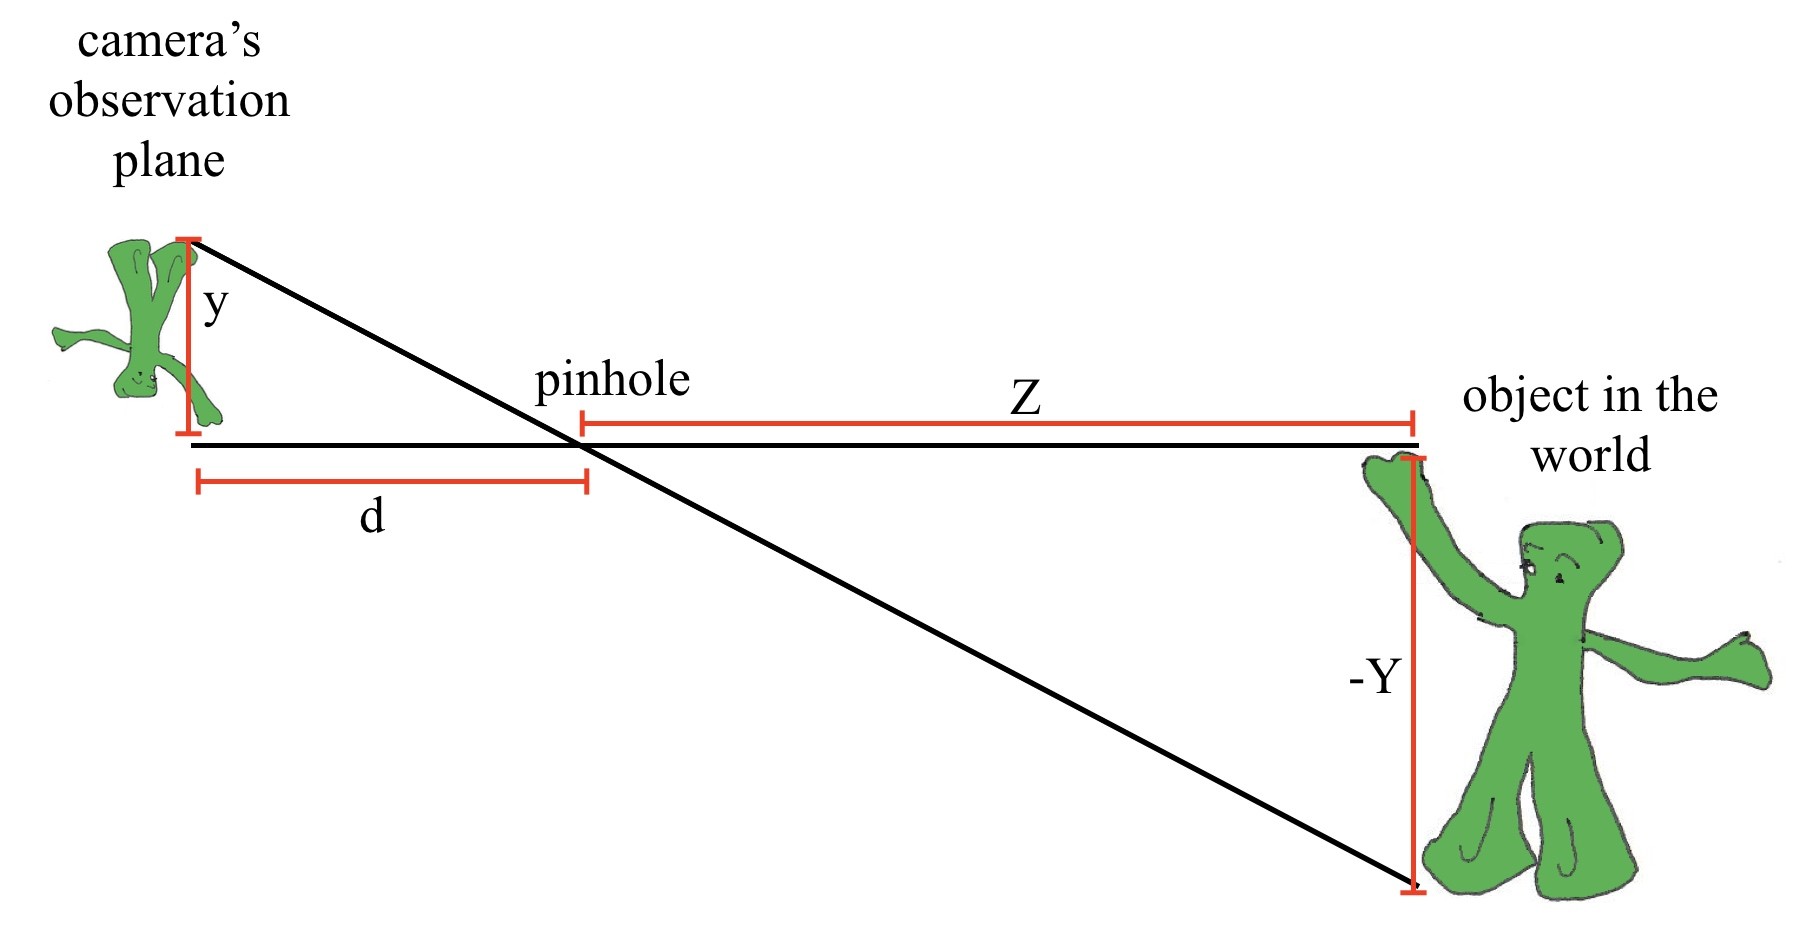
\includegraphics[width=.8\linewidth]{figures/imaging/pinholeGeomGumby.jpg}
\includegraphics[width=0.8\linewidth]{figures/imaging_geometry/camera_centric.eps}
}
\caption{Perspective projection. Remember that from similar triangles, we have $x/f = X/Z$ and $y/f = Y/Z$.}
\label{fig:pinholeGeometry2bis}
\end{figure}



To write points in 3D space in homogeneous coordinates, we add a fourth coordinate to the three coordinates of Euclidean space, as described in \chap{\ref{chapter:geometry_homogeneous}}.
%with the same scaling rules applying as for the case of 2D homogeneous coordinates.
Using homogeneous coordinates, camera projections can be written in a simple form as a matrix multiplication.  Consider a coordinate system with the origin fixed at the center of projection of the camera and the 3D point in homogeneous coordinates, $\mathbf{P}=[X, Y, Z, 1]^\transpose$.

We can verify that the matrix, $\mathbf{K}$, shown below, multiplied by the vector describing the 3D point, $\mathbf{P}$, returns the position of its perspective projection (equation [\ref{eq:perspctiveProj}]):
\begin{eqnarray}
    \mathbf{K} \mathbf{P} & = &
    \begin{bmatrix}
    f & 0 & 0 & 0 \\
    0 & f & 0 & 0 \\
    0 & 0 & 1 & 0
    \end{bmatrix}
    \begin{bmatrix}
    X \\
    Y \\
    Z \\
    1
    \end{bmatrix}
     = 
    \begin{bmatrix}
    f X \\
    f Y \\
    Z
    \end{bmatrix}
    =
    \lambda
    \begin{bmatrix}
    x \\
    y \\
    1
    \end{bmatrix}
\end{eqnarray}
Transforming the product vector from homogeneous coordinates to heterogeneous coordinates yields
\begin{equation}
    \begin{bmatrix}
    f X \\
    f Y \\
    Z
    \end{bmatrix}
    \rightarrow
    \begin{pmatrix}
    f X/Z \\
    f Y/Z
    \end{pmatrix}
    =
    \begin{pmatrix}{c}
    x \\
    y
    \end{pmatrix}
    =
    \mathbf{p}
\end{equation}
showing that the matrix $\mathbf{K}$, when multiplied by the homogeneous coordinates of a 3D point, $\mathbf{P}$, renders the homogeneous coordinates of the perspective projection of that 3D point, $\mathbf{p}$. This formulation is one of the biggest benefits of using homogeneous coordinates. It allows writing perspective projection as a linear operator in homogeneous coordinates.

Because homogeneous coordinates, and therefore also the transformation matrices, are only defined up to an arbitrary uniform (non zero) scale factor, the perspective projection transformation matrix is equivalently written as
\begin{equation}
    \mathbf{K} =             
    \begin{bmatrix}
    1 & 0 & 0 & 0 \\
    0 & 1 & 0 & 0 \\
    0 & 0 & 1/f & 0
    \end{bmatrix}
    \label{eq:homogPerspective}
\end{equation}
Also, in this particular case, it is fine to drop the last column of $\mathbf{K}$ and use the heterogeneous coordinates form of $\mathbf{P}$. However, it is interesting to keep the homogeneous formulation, as it will allow us to work with more general forms of camera models, as we will see next. 



\subsection{Parallel Projection}

We can use homogeneous coordinates to describe a wide variety of camera models.
For instance, the projection matrix for an orthographic projection (equation [\ref{eq:orthographicProj}]), $\mathbf{K}$, is
\begin{equation}
\mathbf{K} =         
    \begin{bmatrix}
    1 & 0 & 0 & 0 \\
    0 & 1 & 0 & 0 \\
    0 & 0 & 0 & 1
    \end{bmatrix}
    ,
    \label{eq:parallel_projection_matrix}
\end{equation}
as can be verified by multiplying by a 3D point in homogeneous coordinates.


\section{Camera-Intrinsic Parameters}

%Now that we have seen how 3D to 2D projection can be modeled using homogeneous coordinates and very simple vector computations, how can we use this to model cameras? We want a

%Cameras will output pixels and there might be other factors such as geometric distortions that will affect the relationship between the 3D scene and the image captured by the camera. 

Now that we have seen how 3D to 2D projection can be effectively modeled using homogeneous coordinates and simple vector computations, let's apply these tools to model cameras.

We want to construct a camera model that captures the image formation process. Cameras translate the world into pixels, but the relationship between the 3D scene and the 2D image captured by the camera is not always straightforward. To start with, the world is measured in units of meters while points in images are measured in pixels. Factors such as geometric distortions can influence this relationship, and we need to account for these elements in our camera model.

\subsection{From Meters to Pixels}

\Fig{\ref{fig:pinhole_and_sensor}} illustrates the image formation process and the image sampling by the sensor. 
We need to account for the perspective projection of the point, $\mathbf{P}$, described in camera coordinates, to pixel coordinates in the sensor plane of the camera.  

\begin{figure}[t]
\centerline{
\includegraphics[width=1\linewidth]{figures/imaging_geometry/pinhole_and_sensor.eps}
}
\caption{An image is projected into the sensor. World coordinates are transformed into pixels at the sensor. The focal length is $f$, and the physical width of the sensor is $w$. The sensor has $N \times M$ pixels.}
\label{fig:pinhole_and_sensor}
\end{figure}



The units of the position in pixel space may be different than those of the world coordinates, which scales the focal length, $f$, in \eqn{\ref{eq:homogPerspective}} to some other value. Let's call that value $a$:
\begin{equation}
    \mathbf{K} =             
    \begin{bmatrix}
    a & 0 & 0 & 0 \\
    0 & a & 0 & 0 \\
    0 & 0 & 1 & 0
    \end{bmatrix}
    \label{eq:intrinsic}
\end{equation}
where the constant $a$ is related to the physical camera parameters in the following way:
\begin{equation}
a = f \, N / w
\end{equation}
where $f$ is the focal length (in meters), $w$ is the width of the sensor in meters, and $N$ is the image width in pixels. The ratio $N/w$ is the number of pixels per meter in the sensor.

Also, the image center might not be the pixel $[0,0]^\transpose$. If the optical axis coincides with the image center, we need to apply a translation so that a 3D point on the optical axis (i.e., $X=Y=0$) projects to $[c_x, c_y]^\transpose$. For example, for an image of size $N \times M$ we will have $c_x=N/2$ and $c_y=M/2$:
\begin{equation}
    \mathbf{K} =             
    \begin{bmatrix}
    a & 0 & c_x & 0 \\
    0 & a & c_y & 0 \\
    0 & 0 & 1 & 0
    \end{bmatrix}
    \label{eq:intrinsic}
\end{equation}
It is also possible that the pixels are not square, in which case we have to account for different scaling along both axis:
\begin{equation}
    \mathbf{K} =             
    \begin{bmatrix}
    a & 0 & c_x & 0 \\
    0 & b & c_y & 0 \\
    0 & 0 & 1 & 0
    \end{bmatrix}
    \label{eq:intrinsic}
\end{equation}
Then, the final transformation from 3D coordinates, $[X,Y,Z]^\transpose$, to image pixels, $[n,m]^\transpose$, has the form: 
\begin{equation}
    \begin{bmatrix}
    a & 0 & c_x & 0 \\
    0 & b & c_y & 0 \\
    0 & 0 & 1 & 0
    \end{bmatrix}
    \begin{bmatrix}
    X \\
    Y \\
    Z \\
    1
    \end{bmatrix}
    \rightarrow
    \begin{pmatrix}
    a X/Z+c_x \\
    b Y/Z+c_y
    \end{pmatrix}
    =
    \begin{pmatrix}
    n \\
    m
    \end{pmatrix}
    \label{eq:intrinsic}
\end{equation}




The signs of $a$ and $b$ can be positive or negative. With the convention used in this book, where the camera optical axis coincides with the $Z$-axis and the camera looks in the direction of positive $Z$, the sign of $a$ has to be negative. If $n$ and $m$ are indices into an array, then the image origin is located at the top-left of the array, which means the signs of $a$ and $b$ will be negative. This is the convention used by Python and OpenCV. \Fig{\ref{fig:conventions}} shows two different common conventions. 


\begin{figure}[t]
\centerline{
\includegraphics[width=1\linewidth]{figures/imaging_geometry/conventions_coordinates.eps}
}
\caption{(a) 3D representation of the image plane. 
(b and c) Two different conventions for the image coordinate systems. In this book we have been using (b).}
\label{fig:conventions}
\end{figure}


\subsection{From Pixels to Rays}
\label{sec:pixel_to_rays}

If you have a calibrated camera, can we derive the equation of the ray that leaves the image at one point? Answering this question, will allow us answering the following one: If we know $Z$ for an image pixel with camera-coordinates $x,y$, can get the point world-coordinates $X$ and $Y$? 

We can relate the point in the image plane, $\mathbf{p}$, with the 3D point $\mathbf{P}$ in world-coordinates. To do this, we will first play a little trick: We will express the 2D point $\mathbf{p}$ in 3D coordinates. We can do this by realizing that the point $\mathbf{p}$ is contained in the image plane which is located at a distance $f$ of the origin along the $Z$-axis (\fig{\ref{fig:coordinate_systems_ray}}).
%, also describing $\mathbf{p}$ also using the 3D coordinates. 
Therefore, in 3D, the 2D point $\mathbf{p}$ is a point located at coordinates $Z_c=f$, where $f$ is the focal length, $X_c=x$, and $Y_c=y$, as illustrated in \fig{\ref{fig:coordinate_systems_ray}}.
%\begin{equation}
%    %\mathbf{p} = 
%    \left (
%    \begin{array}{c}
%    x\\
%    y \\
%    f
%    \end{array}
%    \right )
%\end{equation}


\begin{figure}[h]
\centerline{
%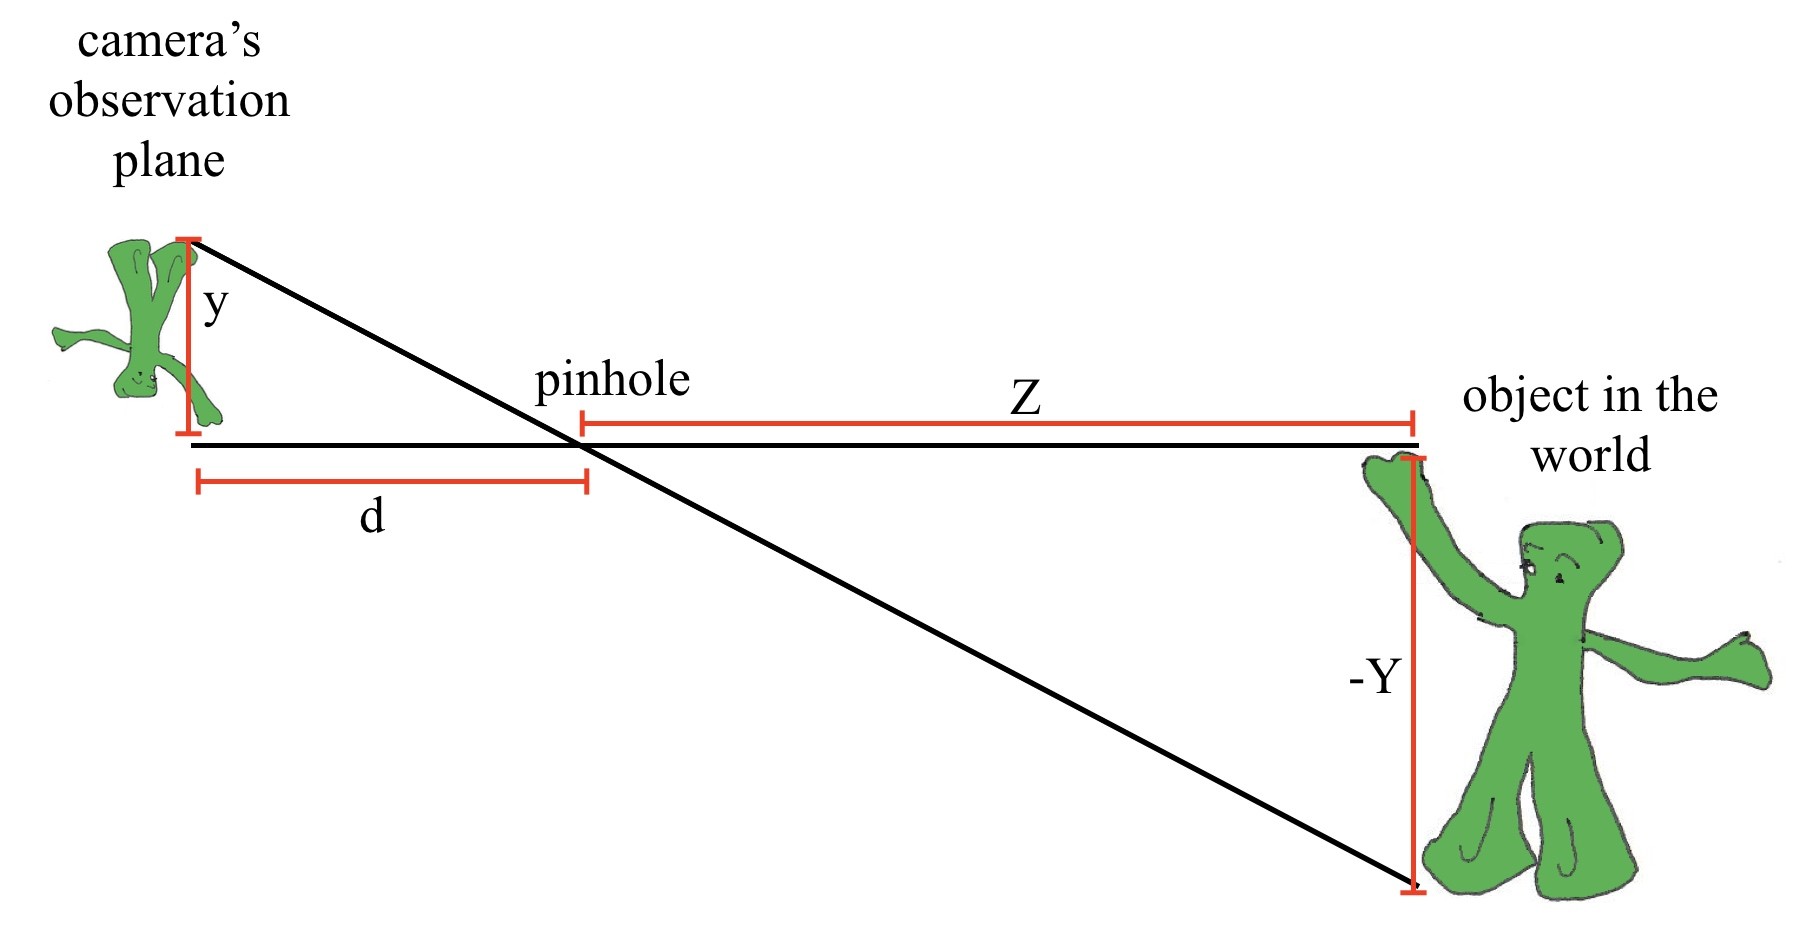
\includegraphics[width=.8\linewidth]{figures/imaging/pinholeGeomGumby.jpg}
\includegraphics[width=0.75\linewidth]{figures/imaging_geometry/light_ray.eps}
}
\caption{The 3D point $\mathbf{P}$ is obtained by scaling the point $\mathbf{p}=(x,y,f)$ with a scaling factor $Z/f$. The ray that passes by the point $\mathbf{p}$ is the line defined by $\lambda (x,y,f)$, with $\lambda$ being a positive real number.}
\label{fig:coordinate_systems_ray}
\end{figure}

The ray that connects the camera center and the point $\mathbf{p}$ is $\lambda (x,y,f)$, with $\lambda$ being a positive real number. Any 3D point along this line will project into the same image point $\mathbf{p}$ under perspective projection. 

As shown in \fig{\ref{fig:coordinate_systems_ray}} the 3D point $\mathbf{P}$ is obtained by scaling the ray that passes by $\mathbf{p}$. The scaling factor is $\lambda = Z/f$:
\begin{equation}
    \frac{Z}{f}
    \begin{pmatrix}
    x\\
    y\\
    f
    \end{pmatrix}
    =
    \begin{pmatrix}
    X \\
    Y \\
    Z
    \end{pmatrix}
\end{equation}

%By changing the value of $Z$ we have the ray that passes by $\mathbf{p}$. 
We should use $a$ instead of $f$ if we are using coordinates in pixels. We will revisit this again in \chap{\ref{chapter:3D_learning_from_single_image}}.


\subsection{A Simple, although Unreliable, Calibration Method}
\label{sec:simple_unreliable_calibration_method}

Everything we described up to here, relies on a series of parameters (i.e., focal length, sensor size) that will be unknown in general. Before we continue, let's try to see if we can find out what those parameters are in a real setting. 

Let's start by describing a simple and intuitive method for camera calibration illustrated in \fig{\ref{fig:simple_calibration}}. The method we will describe is not very accurate, but it provides be a good sanity check before doing more precise camera calibrations. We will describe a more accurate method in \sect{\ref{sec:camera_calibration}}.


\begin{figure}[h]
\centerline{
\sublabel{a}{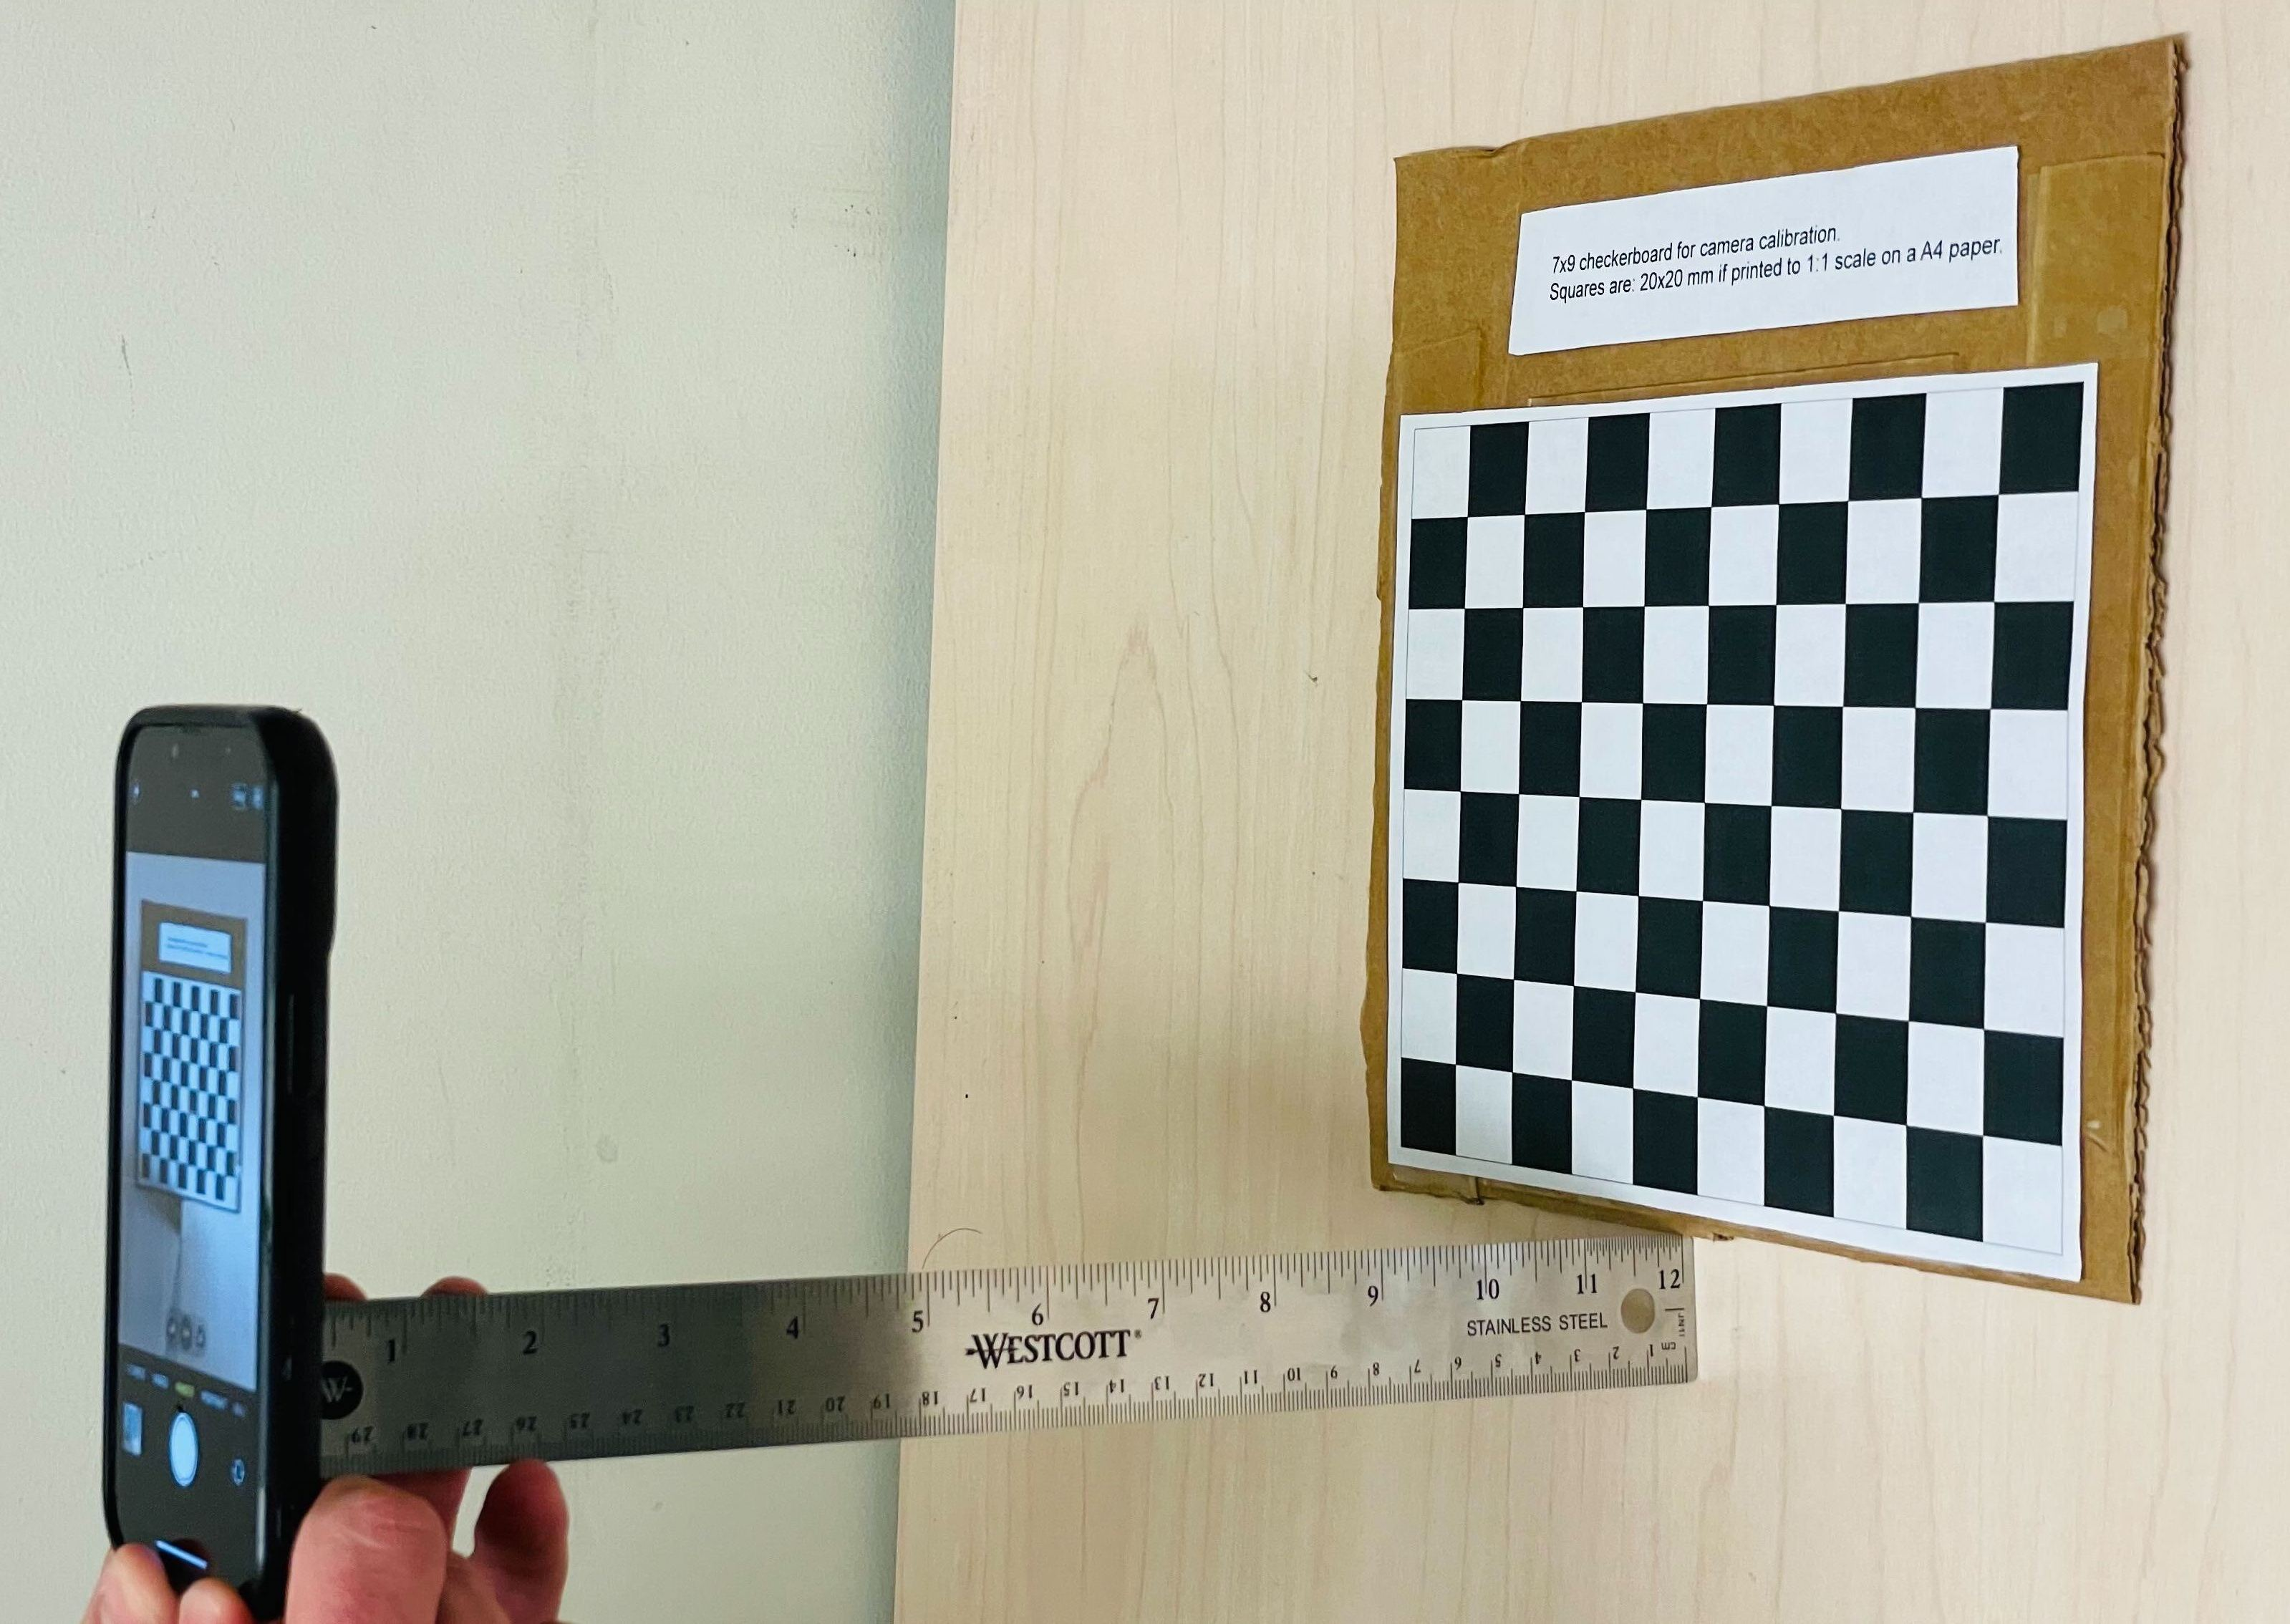
\includegraphics[width=.62\linewidth]{figures/imaging_geometry/simple_calibration_1.jpg}}
%~
\sublabel{b}{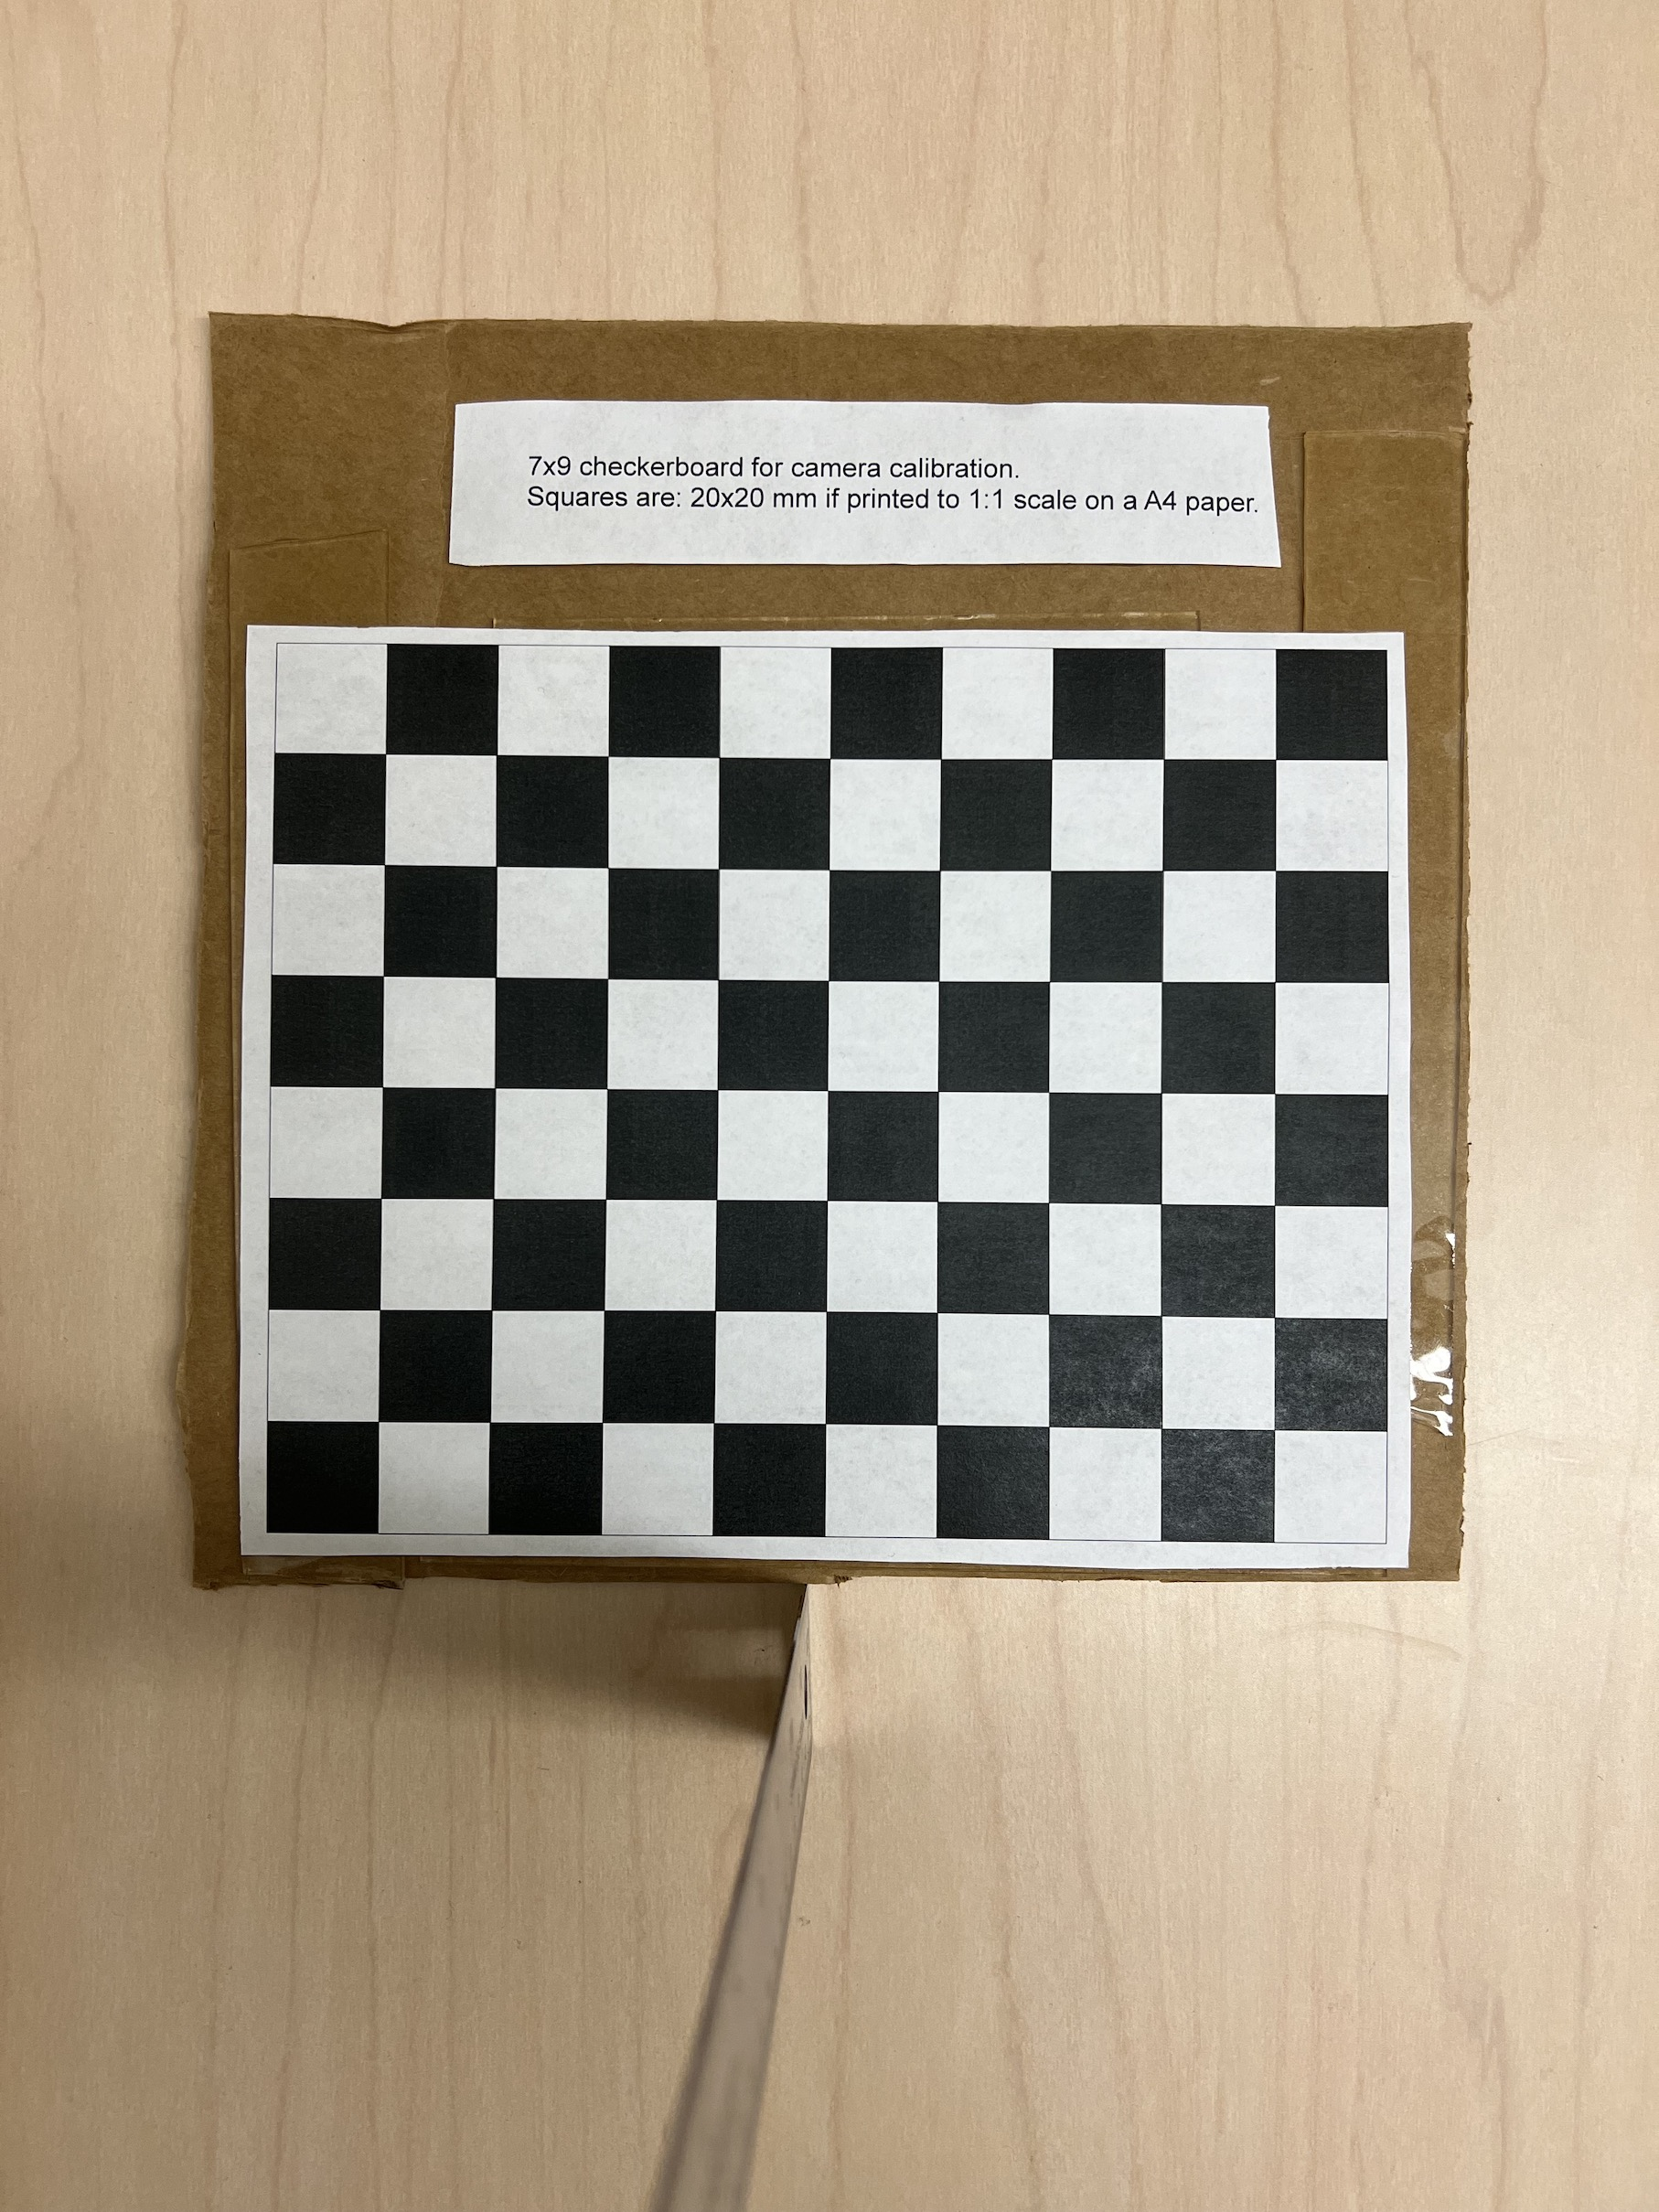
\includegraphics[width=.33\linewidth]{figures/imaging_geometry/simple_calibration_2.jpg}}
}
\caption{A simple calibration setting.}
\label{fig:simple_calibration}
\end{figure}

To calibrate a camera we need the following three ingredients: 
\begin{itemize}
\item An object of known size: In this setting, \fig{\ref{fig:simple_calibration}}{a}, the object is a $8\times10$ chessboard pattern printed so that each square exactly measures 2 $\times$ 2 cm. The total width is $W=20$ cm. This chessboard is a standard calibration target \cite{Zhang1999}. 
\item The distance between the camera and the object: We use a ruler to measure that the distance between the camera and the chessboard as shown in \fig{\ref{fig:simple_calibration}}{a}. The distance is approximately $Z=31$ cm.
\item A picture of the object: \Fig{\ref{fig:simple_calibration}}{b} shows the picture taken by the camera shown in \fig{\ref{fig:simple_calibration}}{a}. The camera plane is parallel to the chessboard. From the picture, we can measure the width of the chessboard in pixels, which is $L=2{,}002$ pixels. 
\end{itemize}
These three quantities, $W$, $L$ and $Z$, are related via the parameter $a$ of the projection matrix by the equation: $a= Z L/W$, which results in:
\begin{equation}
a = \frac{31 \times 2{,}002}{20} = 3{,}103.1
\end{equation}

%to take a picture of an object of a known size from a known distance and use the size of the object measured on the image to calculate the camera parameters. The following image shows an example of this calibration setting:

% https://www.analyticsvidhya.com/blog/2021/10/a-comprehensive-guide-for-camera-calibration-in-computer-vision/





%In this setting, \fig{\ref{fig:simple_calibration}}, the object is a $8\times10$ checkerboard pattern printed so that each square exactly measures 2cm $\times$ 2cm. The picture is taken with a phone camera placed so that the camera plane is parallel to the checkerboard.
% https://forums.macrumors.com/threads/flagship-camera-comparison-13-pro-12-pro-max-12-pro-11-pro-xs-x.2311859/?fr=operanews

%\marginnote{Geometry corresponding to \fig{\ref{fig:simple_calibration}}:\\
%\centerline{
%\includegraphics[width=1\linewidth]{figures/imaging_geometry/calibration_a.eps}}
%}
%The left image in \fig{\ref{fig:simple_calibration}} shows the overall configuration were the phone is used to take a picture of a calibration board. The intrinsic parameter $a$ can be estimated as $a= Z L/W$ where $Z$ is the distance to the board, $W$ is the board width and $L$ is the width of the board in pixels in the picture. The board is a checkerboard with a width of 20cm. The camera is approximately fronto-parallel to the board and at a distance of 31cm to it.  

The picture size is $4{,}032 \times 3{,}024$ pixels which we can use to get the other two parameters of the camera projection matrix: $c_x=3{,}024/2$ and $c_y=4{,}032/2$. Putting all together we get the projection matrix:

\begin{equation}
    \mathbf{K} =             
    \begin{bmatrix}
    3{,}103.1 & 0 & 1{,}512 & 0 \\
    0 & 3{,}103.1 & 2{,}016 & 0 \\
    0 & 0 & 1 & 0
    \end{bmatrix}
    \label{eq:intrinsic}
\end{equation}

Would it be possible to infer the intrisic camera matrix from the camera technical specifications alone?  Can we directly estimate the parameter $a$ directly from the camera specs? The picture is taken with the wide-angle lens of an iPhone 13 pro. The focal length is 5.7 mm, the sensor size is $7.6 \times 5.7$ mm, and the image size is $4{,}032 \times 3{,}024$ pixels. This gives as an intrinsic parameter of:
\begin{equation}
a = \frac{4{,}032 \times 5.7}{7.6} = 3{,}024. 
\end{equation}
It works! (Does it?) Or at least it is close. But a lot of things happen inside a camera and estimating these values from hardware specs might be difficult.

But is this quality for the calibration enough? 


\subsection{Other Camera Parameters}

Unfortunately, there are other important aspects of a camera that require precise calibration. In some rare cases, pixels might not be square, or might be arranged along non-perpendicular axes, which requires introducing a skew parameter in $\mathbf{K}$. 
Radial distortion introduced by lenses is often an important and frequent source of issues that requires calibration. When there is radial distortion, straight lines will appear curved. In that case, it is very important to correct for the distortion. Standardized tools for camera calibrations take into account all these different aspects of the camera in order to build an accurate camera model. A more in-depth description of these tools and methods can be found here \cite{Zhang1999,Zhang2000}.



%\section{Camera model}
\section{Camera-Extrinsic Parameters}

In all our previous examples, we have been assuming that the camera origin was located at the origin of the world coordinate system with the optical axis aligned with the world $Z$-axis. In practice, there will be many situations where placing the camera at a special position will be more convenient. For instance, in the simple vision system we studied in chapter \ref{chapter:simplesystem} the camera center was placed above the $Z$-axis. Let's now study a more general setup where the camera is placed at an arbitrary location away from the world coordinate system. 

In the examples shown in \fig{\ref{fig:camera_calibration}}, we are interested in placing the world coordinate system so that the origin is on the ground and the axes $Z_w$ and $X_W$ are contained on the ground plane, and parallel to the two axis defined by the table. The axis $Y_W$ is perpendicular to the ground. Let's say that our camera has its camera center displaced by vector $\mathbf{T}$ and the axes are rotated by $\mathbf{R}^\transpose$ with respect to the world-coordinates system, as shown in \fig{\ref{fig:camera_calibration}}. Precisely, this is done by first placing the camera at the origin of the world-coordinates system, then rotating the camera with the rotation matrix $\mathbf{R}^\transpose$ and finally translating it by $\mathbf{T}$ (the order of these two operations matters). We use the inverse of $\mathbf{R}$ (equal to its transpose) to simplify the derivations later. 



\begin{figure}[t]
\centerline{
\includegraphics[width=0.7\linewidth]{figures/imaging_geometry/world_and_camera_coordinates_2.eps}
}
\caption{World- and camera-coordinate systems. A 3D point expressed in world coordinates, $\mathbf{P}_W$, can be expressed in the camera-coordinate frame, $\mathbf{P}_c$, by applying the translation, $\mathbf{T}$, and rotation, $\mathbf{R}$, to the point coordinates.}
\label{fig:camera_calibration}
\end{figure}

We are now given a point in the world $\mathbf{P}_W$, with its coordinates are described in terms of the world-coordinate system. Our goal is to find how that point projects into the image captured by the camera. To do this, first we need to change the coordinate system and express the point with respect to the camera coordinate system. Once we have done that change of coordinate system, we can use the intrinsic camera model $K$ to project the point into the image plane.  


%In order to compute the projection of this point into the camera we will do this in two steps.



%We need to translate, and then to rotate the camera so that points in the world, $\mathbf{P}_W$, are written in terms of a coordinate system with its origin at the camera center, and rotated to align with the camera (note that the order is reverse to how we defined the camera coordinate system earlier in this section). 

We need to initially translate, and subsequently rotate, the camera so that points in the world, $\mathbf{P}_W$, are expressed in a coordinate system that originates at the camera center and is rotated to align with the camera. Note that this order is reversed from how we defined the camera coordinate system earlier in this section. Using heterogeneous coordinates we can describe these two transformations as:

\begin{equation}
\mathbf{P}_C = \mathbf{R} (\mathbf{P}_W  - \mathbf{T}) = \mathbf{R} \mathbf{P}_W  -  \mathbf{R}\mathbf{T}
\end{equation}
where we use the $3\times3$ matrix, $\mathbf{R}$, to rotate the camera so that the camera's coordinates are parallel to those of the world. The vector $\mathbf{T}$ is the position of the camera in world coordinates. The rotation $\mathbf{R}$ in this equation is the inverse of the rotation matrix of the camera coordinate system with respect to the world coordinates.

%If we do translation and then rotation we would get $\mathbf{R} ( \mathbf{P}_W  - \mathbf{T})$. 



Let's use now homogeneous coordinates to describe the transformation from world coordinates to camera coordinates. To do so, we first translate the coordinate system by $-\mathbf{T}$ using the homogeneous matrix, $\mathbf{M}_1$:

\begin{equation}
\mathbf{M}_1 =         
    \begin{bmatrix}
    1 & 0 & 0 & -T_X \\
    0 & 1 & 0 & -T_Y \\
    0 & 0 & 1 & -T_Z \\
    0 & 0 & 0 & 1
    \end{bmatrix}
\end{equation}

Then, we use the $3\times 3$ matrix, $\mathbf{R}$, to rotate the camera so that the camera's coordinates are parallel to those of the world:
\begin{equation}
\mathbf{M}_2 =         
    \begin{bmatrix}
    R_1 & R_2 & R_3  & 0 \\
    R_4 & R_5 & R_6 & 0 \\
    R_7 & R_8 & R_9 & 0 \\
    0 & 0 & 0 & 1
    \end{bmatrix}
    \label{eq:homographyRotation}
\end{equation}


Using these two matrices we have
\begin{equation}
\mathbf{P}_C = \mathbf{M}_2 \mathbf{M}_1 \mathbf{P}_W
\label{eq:extrinsic}
\end{equation}
where $\mathbf{P}_W$ and $\mathbf{P}_C$ are the 3D coordinates of the same point (\fig{\ref{fig:camera_calibration}}), written in world and camera coordinates, respectively. Sometimes, this transformation is written by making the product of the two matrices explicit:

\begin{equation}
\mathbf{M}_2 \mathbf{M}_1=         
    \begin{bmatrix}
    R_1 & R_2 & R_3  & -\mathbf{r}_1 \mathbf{T} \\
    R_4 & R_5 & R_6 & - \mathbf{r}_2 \mathbf{T} \\
    R_7 & R_8 & R_9 & - \mathbf{r}_3 \mathbf{T} \\
    0 & 0 & 0 & 1
    \end{bmatrix}
    =
    \begin{bmatrix}
    \mathbf{R} & -\mathbf{R}\mathbf{T} \\
    \mathbf{0}^\transpose & 1
    \end{bmatrix}
\label{eq:extrinsic2}
\end{equation}
where $\mathbf{r}_i$ represents the row $i$ of the rotation matrix $\mathbf{R}$. 

Substituting \eqn{\ref{eq:extrinsic2}} into \eqn{\ref{eq:extrinsic}} we can now translate a 3D point expressed in world coordinates into camera coordinates:
\begin{equation}
\mathbf{P}_C = 
    \begin{bmatrix}
    \mathbf{R} & -\mathbf{R}\mathbf{T} \\
    \mathbf{0}^\transpose & 1
    \end{bmatrix}
    \mathbf{P}_W
%\label{eq:extrinsic}
\end{equation}

The camera parameters, $\mathbf{R}$ and $\mathbf{T}$, that relate the camera to the world are called the {\bf extrinsic camera parameters}. These parameters are external to the camera. 

We have seen now how to transform a point described in the world-coordinate system into the camera-coordinates system. We can now use the intrinsic camera parameters to project the point into the image plane. In the next section we will see how to combine both sets of parameters to get a full camera model. 



\section{Full Camera Model}

The concatenation of the extrinsic and intrinsic transformation matrices yields the desired transformation matrix, which will transform world coordinates to rendered pixel coordinates:
\begin{equation}
    \lambda
    \begin{bmatrix}
    x \\
    y \\
    1
    \end{bmatrix}
    =
    \begin{bmatrix}
    x' \\
    y' \\
    w
    \end{bmatrix}
=
\mathbf{K} \mathbf{M}_2 \mathbf{M}_1 
    \begin{bmatrix}
    X \\
    Y \\
    Z \\
    1
    \end{bmatrix}
    \label{eq:combined}
\end{equation}
Converting back to heterogeneous from homogeneous coordinates, the 2D pixel indices of a 3D point $[X, Y, Z]^\transpose$ are $[x,y]^\transpose=[x'/w, y'/w]^\transpose$. 
%Writing this out, we have, for the case of a camera (square pixels), with general extrinsic parameters, the expression to transform from 3D position to the measured sensor position of that 3D point:
We can make all the matrices in \eqn{\ref{eq:combined}} explicit and write:
\begin{equation}
    \begin{bmatrix}
    x' \\
    y' \\
    w
    \end{bmatrix}
=
    \begin{bmatrix}
    a & 0 & c_x & 0 \\
    0 & a & c_y & 0 \\
    0 & 0 & 1 & 0
    \end{bmatrix}
    \begin{bmatrix}
    R_1 & R_2 & R_3  & 0 \\
    R_4 & R_5 & R_6 & 0 \\
    R_7 & R_8 & R_9 & 0 \\
    0 & 0 & 0 & 1
    \end{bmatrix}
    \begin{bmatrix}
    1 & 0 & 0 & -T_X \\
    0 & 1 & 0 & -T_Y \\
    0 & 0 & 1 & -T_Z \\
    0 & 0 & 0 & 1
    \end{bmatrix}
    \begin{bmatrix}
    X \\
    Y \\
    Z \\
    1
    \end{bmatrix}
    \label{eq:combinedexpanded}
\end{equation}


The right-most matrix multiplications reflect the camera's extrinsic parameters, and the left-most matrix reflects the intrinsic parameters and the perspective projection.  Note that column of zeros in the left-most matrix means that, without loss of generality, \eqn{\ref{eq:combinedexpanded}} can be written in slightly simpler form as:
\begin{equation}
    \begin{bmatrix}
    x' \\
    y' \\
    w
    \end{bmatrix}
=
    \begin{bmatrix}
    a & 0 & c_x  \\
    0 & a & c_y  \\
    0 & 0 & 1 
    \end{bmatrix}
    \begin{bmatrix}
    R_1 & R_2 & R_3   \\
    R_4 & R_5 & R_6  \\
    R_7 & R_8 & R_9 
    \end{bmatrix}
    \begin{bmatrix}
    1 & 0 & 0 & -T_X \\
    0 & 1 & 0 & -T_Y \\
    0 & 0 & 1 & -T_Z
    \end{bmatrix}
    \begin{bmatrix}
    X \\
    Y \\
    Z \\
    1
    \end{bmatrix}
    \label{eq:combinedexpandedsmaller}
\end{equation}

This is usually written as:
\begin{equation}
\mathbf{p} = 
    \mathbf{K}
    %\left [
    %\begin{array}{cc}
    %\mathbf{R} & -\mathbf{R} \mathbf{T}
    %\end{array}
    %\right ]
    \begin{bmatrix}
    \mathbf{R} ~ \vline ~ -\mathbf{R} \mathbf{T} 
    \end{bmatrix}
    \mathbf{P}_W 
%\label{eq:extrinsic}
\end{equation}


By replacing $\mathbf{K}$ with different intrinsic parameters we can build models for different camera types such as orthographic cameras, weak-perspective model, affine cameras, and so on. \Fig{\ref{fig:summary_camera_projection}} summarizes this section.


\begin{figure}[t]
\centerline{
\includegraphics[width=0.8\linewidth]{figures/imaging_geometry/summary_camera_model.eps}
}
\caption{Projection of a point into the image plane. This summary puts together \fig{\ref{fig:pinholeGeometry2bis}} and \fig{\ref{fig:camera_calibration}}. First, we change the world-coordinates system, in which the point is expressed, into the camera-coordinates system, using the extrinsic camera model, and then we project it into the camera plane using the intrinsic camera model.}
\label{fig:summary_camera_projection}
\end{figure}


In the rest, we will usually refer to the camera projection matrix, which includes both intrinsic as extrinsic parameters as:
\begin{equation}
    \mathbf{M} = 
    \mathbf{K}
    \begin{bmatrix}
    \mathbf{R} & -\mathbf{R}\mathbf{T} \\
    \mathbf{0}^T & 1
    \end{bmatrix}
\label{eq:projection_matrix}
\end{equation}

\section{A Few Concrete Examples}

Let's write down the full camera model for a few concrete scenarios that are also of practical relevance. The four scenarios we will consider have growing complexity as shown in \fig{\ref{fig:camera_calibration_scenarios}}.


\begin{figure}
\centerline{
\includegraphics[width=1\linewidth]{figures/imaging_geometry/camera_calibration_scenarios.eps}
}
\caption{Four examples of camera poses respect to the world-coordinates system with increasing complexity. In the text we derive the projection matrix for each scenario.}
\label{fig:camera_calibration_scenarios}
\end{figure}

\noindent {\bf Example 1}. We will start with a camera located at the origin of the world-coordinate systems, as shown in \fig{\ref{fig:camera_calibration_scenarios}}{a}. In this case, both coordinate systems are identical and the camera projection matrix is:

\begin{equation}
    \mathbf{M} 
    =             
    \begin{bmatrix}
    a & 0 & 0 & 0 \\
    0 & a & 0 & 0 \\
    0 & 0 & 1 & 0
    \end{bmatrix}
    \begin{bmatrix}
    1 & 0 & 0 & 0 \\
    0 & 1 & 0 & 0 \\
    0 & 0 & 1 & 0 \\
    0 & 0 & 0 & 1 \\
    \end{bmatrix}
    =
    \begin{bmatrix}
    a & 0 & 0 & 0 \\
    0 & a & 0 & 0 \\
    0 & 0 & 1 & 0
    \end{bmatrix}
    \label{eq:model1}
\end{equation}

We have set $c_x=c_y=0$, which assumes that the center of the image are the coordinates $(x,y)=(0,0)$. This will simplify the equations for the following examples. 


\noindent {\bf Example 2}. The second scenario we will consider is shown in \fig{\ref{fig:camera_calibration_scenarios}}{b}. This scenario corresponds to a case where a person is holding a camera, pointing toward the horizon in such a way that the optical axis of the camera is parallel to the ground. In this case we place the world-coordinate frame with its origin on the ground plane right below the camera. The camera is at a height $h$ from the ground, measured in meters. 


\begin{equation}
    \mathbf{M} 
    =             
    \begin{bmatrix}
    a & 0 & 0 & 0 \\
    0 & a & 0 & 0 \\
    0 & 0 & 1 & 0
    \end{bmatrix}
    \begin{bmatrix}
    1 & 0 & 0 & 0 \\
    0 & 1 & 0 & -h \\
    0 & 0 & 1 & 0 \\
    0 & 0 & 0 & 1 \\
    \end{bmatrix}
    =
    \begin{bmatrix}
    a & 0 & 0 & 0 \\
    0 & a & 0 & -ah \\
    0 & 0 & 1 & 0
    \end{bmatrix}
    \label{eq:model2}
\end{equation}

Going back to heterogeneous coordinates we have that a 3D point at location $P_W=[X, Y, Z]^\transpose$ in world coordinates projects to the image coordinates:
\begin{eqnarray}
x &=& a \frac{X}{Z} \\
y &=& a \frac{Y-h}{Z} 
\end{eqnarray}
In this scenario, if you hold the camera parallel to the ground at the height of your eyes and take a picture of a person standing in front of you with a similar height, their eyes will project near the middle portion of the vertical axis of the picture (their eyes will be located at $Y\simeq h$; therefore, they will project to $y \simeq 0$, which is the center of the picture). And this will be true regardless of how far away they are. This is illustrated in \fig{\ref{fig:horizon_heads}}. The horizon line is located at the points where $Z \rightarrow \infty$, which are also at $y=0$ (we will talk more about the horizon line in the following chapter). 


\begin{figure}[t]
\centerline{
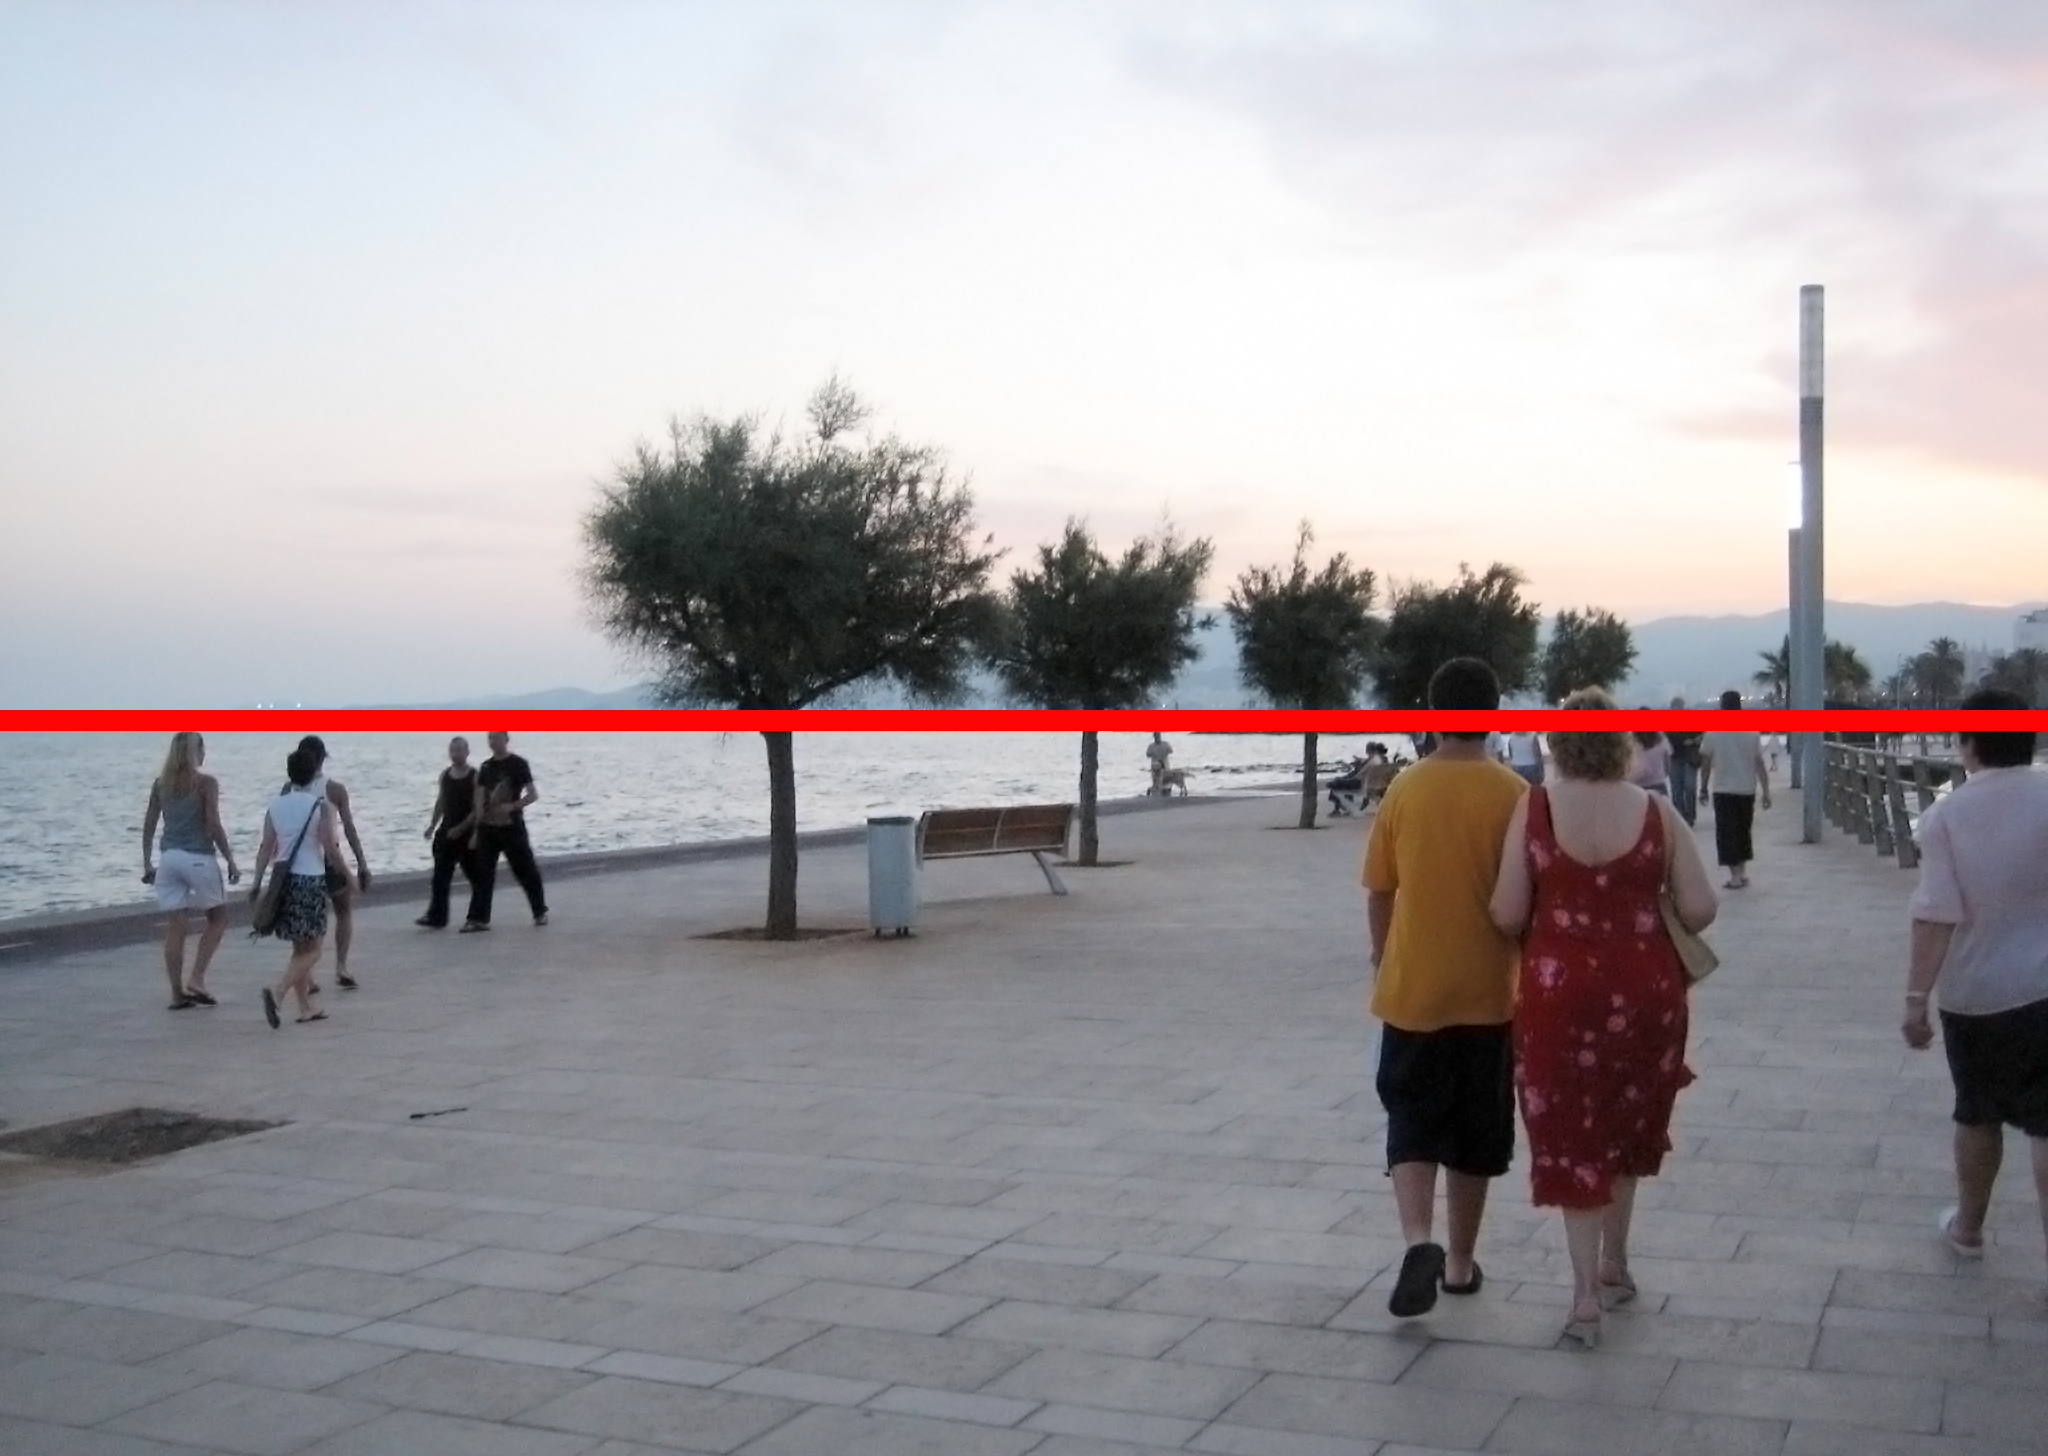
\includegraphics[width=.6\linewidth]{figures/imaging_geometry/horizon_heads.jpg}
}
\caption{If you hold the camera parallel to the ground at the height of your eyes and take a picture of a person standing in front of you with a similar height, their eyes will project near the middle portion of the vertical axis of the picture.}
\label{fig:horizon_heads}
\end{figure}

\noindent {\bf Example 3}. Let's now consider that the camera is tilted by looking downward with an angle $\theta$, as shown in \fig{\ref{fig:camera_calibration_scenarios}}{c}. The horizontal camera axis remains parallel to the ground, but now the optical axis points toward the ground if $\theta>0$. 


Let's first write down the camera-extrinsic parameters. The angle $\theta$ here corresponds to a rotation around the $X_c$-axis, thus we can write:
\begin{eqnarray}
    \begin{bmatrix}
    \mathbf{R} & -\mathbf{R}\mathbf{T} \\
    \mathbf{0}^\transpose & 1
    \end{bmatrix}
    &=&        
    \begin{bmatrix}
    1 & 0 & 0 & 0 \\
    0 & \cos (\theta) & \sin (\theta) & 0 \\
    0 & -\sin (\theta) & \cos (\theta) & 0 \\
    0 & 0 & 0 & 1 \\
    \end{bmatrix}
    \begin{bmatrix}
    1 & 0 & 0 & 0 \\
    0 & 1 & 0 & -h \\
    0 & 0 & 1 & 0 \\
    0 & 0 & 0 & 1 \\
    \end{bmatrix}
    \\
    &=&
    \begin{bmatrix}
    1 & 0 & 0 & 0 \\
    0 & \cos (\theta) & \sin (\theta) & -h \cos (\theta) \\
    0 & -\sin (\theta) & \cos (\theta) & h \sin (\theta) \\
    0 & 0 & 0 & 1 \\
    \end{bmatrix}
    \label{eq:model3}
\end{eqnarray}

Putting both intrinsic and extrinsic camera parameters together we get the following projection matrix:
\begin{eqnarray}
    \mathbf{M} 
%    &=&             
%    \left [
%    \begin{array}{cccc}
%    a & 0 & 0 & 0 \\
%    0 & a & 0 & 0 \\
%    0 & 0 & 1 & 0
%    \end{array}
%    \right ]
%    \left [
%    \begin{array}{cccc}
%    1 & 0 & 0 & 0 \\
%    0 & \cos (\theta) & -\sin (\theta) & -h \cos (\theta) \\
%    0 & \sin (\theta) & \cos (\theta) & -h \sin (\theta) \\
%    0 & 0 & 0 & 1 \\
%    \end{array}
%    \right ] \nonumber \\
    &=& 
    \begin{bmatrix}
    a & 0 & 0 & 0 \\
    0 & a\cos (\theta) & a\sin (\theta) & -ah \cos (\theta) \\
    0 & -\sin (\theta) & \cos (\theta) & h \sin (\theta) \\
    \end{bmatrix}
    \label{eq:model3b}
\end{eqnarray}

Going back to heterogeneous coordinates we have:
%\begin{eqnarray}
%x &=& a \frac{X}{-\sin( \theta ) Y + \cos ( \theta ) Z + h \sin (\theta)} \\
%y &=& a \frac{\cos (\theta) Y + \sin(\theta)Z - h\cos(\theta)}{-\sin( \theta ) Y + \cos ( \theta ) Z + h \sin (\theta)} 
%\end{eqnarray}

\begin{eqnarray}
x &=& a \frac{X}{\sin( \theta ) (h-Y) + \cos ( \theta ) Z} \\
y &=& a \frac{\cos (\theta) (Y-h) + \sin(\theta)Z}{\sin( \theta ) (h-Y) + \cos ( \theta ) Z} \label{eqn:model3camera}
\end{eqnarray}
%  Person Throwing a Stone at a Bird, 1926 by Joan Miro 
% https://www.joan-miro.net/person-throwing-a-stone-at-a-bird.jsp

Let's look at three special cases according to the camera angle $\theta$:
\begin{itemize}
\item For $\theta=0$, we recover the projection equations from the previous example. The horizon line is an horizontal line that passes by the center of the image. 

\item For $\theta=90$ degrees (this is when the camera is looking downward), we get $x=a X / (h-Y)$ and $y=a Z/(h-Y)$. In this case, the equations are analogous to the standard projection equation with the distance to the camera being $h-Y$ and $Z$ playing the role of $Y$.

\item For arbitrary angles $\theta$, 
the horizon line corresponds to the $y$ location for a point in infinity, $Z \rightarrow \infty$. Using \eqn{\ref{eqn:model3camera}}, the horizon line is located at $y = a \tan(\theta)$.  
\end{itemize}
%is located at the point where $Z \rightarrow \infty$ which will be located at $y = a \tan(\theta)$. 

The sketch in \fig{\ref{fig:sketch_eyes_location}} shows a person taking a picture of two people standing at different distances from the camera. If you take a picture of two people with a similar height to you, $h$, standing in front of the camera. Then, we can set $Y=h$ in the previous equations, their eyes will be located at the position $y = a \tan(\theta)$ in the picture, which is independent of $Z$ and the same vertical location as the horizon line. 

\begin{figure}[t]
\centerline{
\includegraphics[width=.9\linewidth]{figures/imaging_geometry/eyes_location.eps}
}
\caption{Sketch showing a person taking a picture of two people standing at different distances from the camera. Their eyes will project to the same image row regardless of their distance to the camera.}
\label{fig:sketch_eyes_location}
\end{figure}

Note that if $a$ is known (i.e., if the camera is calibrated), then we can infer $\theta$ by locating the horizon line in the image. Analogously, if the angle of the camera, $\theta$, is known, we could estimate $a$.

% Image with horizon high: 20 degrees (camera pointing down) horizon_line = 2641- 3024/2 = 1129
% image with horizon low: angle = 14.6 degrees (camera pointing up) horizon_line = 714- 3024/2 = -798

The two pictures in \fig{\ref{fig:low_and_high_horizon}} are taken with two different camera angles. In both pictures, the camera's $x$-axis is kept parallel to the ground. The right and left pictures were taken at the same location with the camera tilted upward and downward, respectively. The horizontal red lines show the approximate location of the horizon line in each image and coincides also with the vertical location where the heads of the people walking appear on the picture. 

\begin{figure}[t]
\centerline{
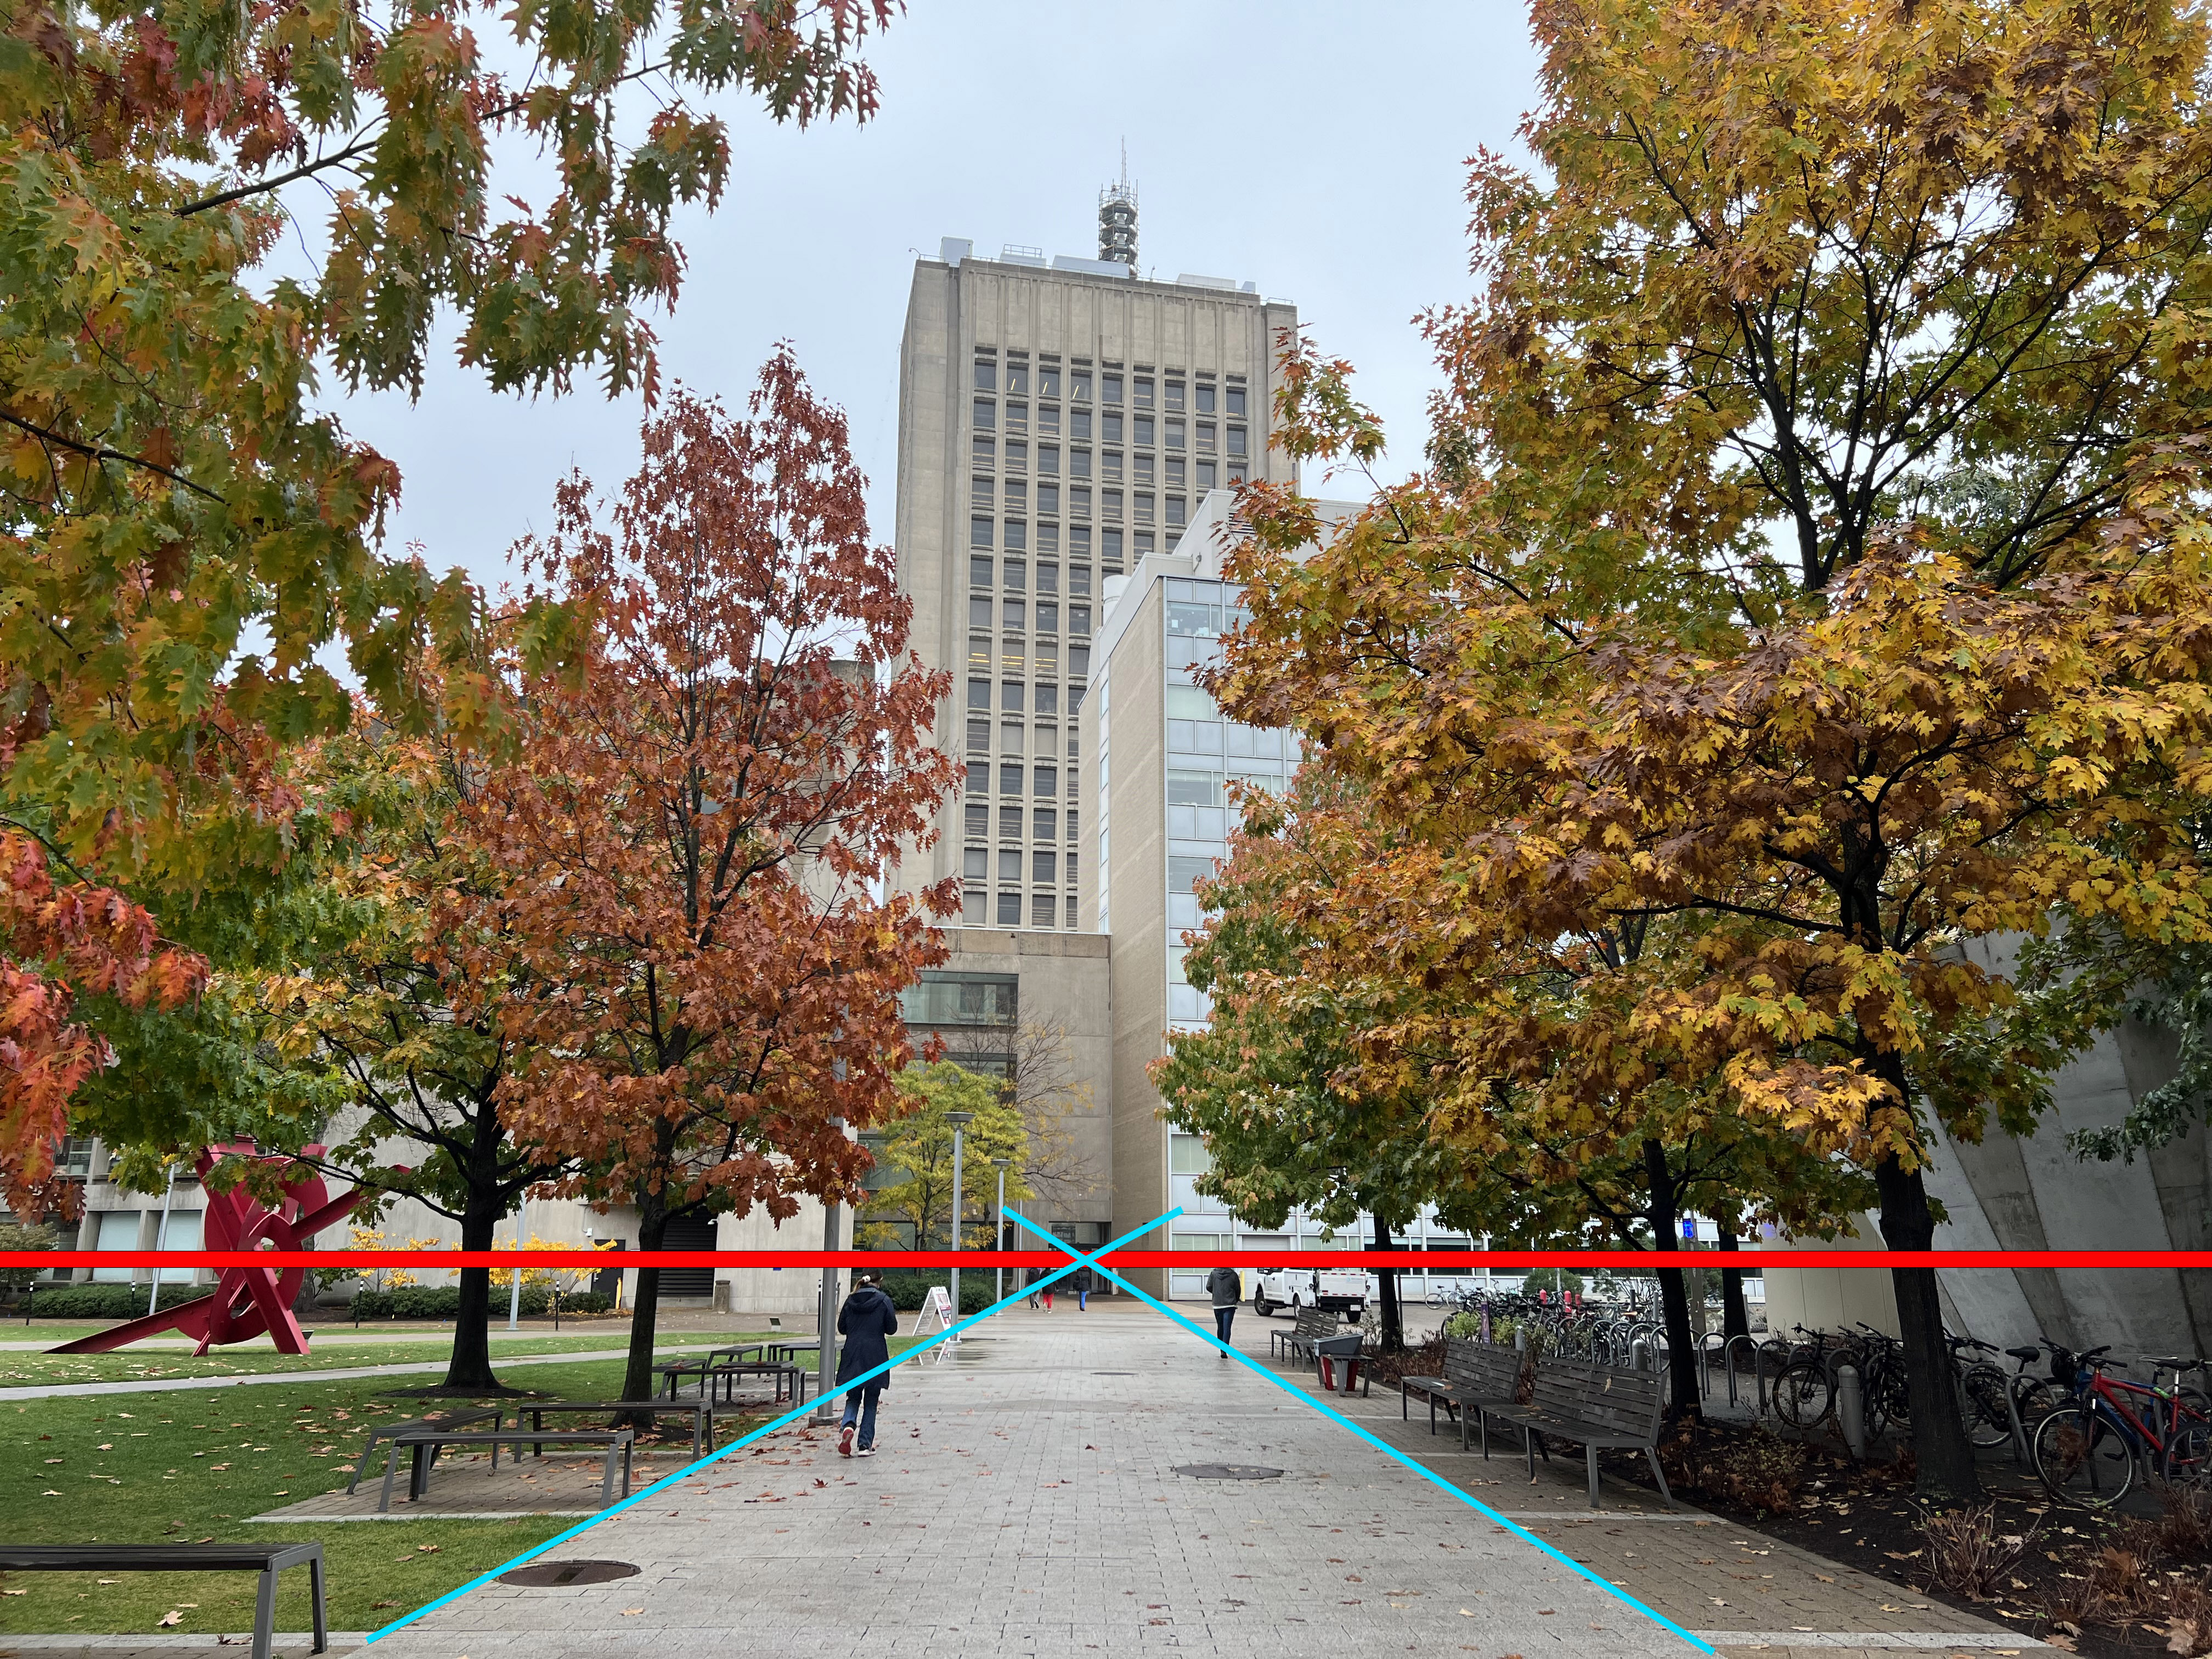
\includegraphics[width=.48\linewidth]{figures/imaging_geometry/low_horizon_vp.jpg}
~
\includegraphics[width=.48\linewidth]{figures/imaging_geometry/high_horizon_vp.jpg}
}
\caption{The two pictures taken with two different camera angles. The red line indicates the position of the horizon line estimated as the horizontal location in which the two vanishing lines (blue) intersect.}
\label{fig:low_and_high_horizon}
\end{figure}

These pictures were taken with the iPhone 13 pro, which we calibrated before. The intrinsic camera parameter we got is $a  \simeq 3{,}103$, which we can use to compute the angle $\theta$. On the right, the location of the horizon line is at $y_h=-798$, with the center of the picture being the coordinates ($0,0$). The angle is $\theta = \arctan (y_h/a)=14.6$ degrees. For the picture on the right the horizon line is at $y_h=1{,}129$, resulting in an estimated camera angle of $\theta=20$ degrees. Although we did not precisely measured the angle of the camera when we were taking these two pictures, both angles seem about right. We leave it to the reader to take two similar pictures to the ones in the example above, and get a precise measurement of the camera angle using a protractor and check if the estimated angle from the horizon line matches your measurement.  

\marginnote{Example 3 can be useful to model typical imaging conditions. It results in a simple model with three parameters ($h$, $a$, and $\theta$). }

\noindent {\bf Example 4}. The setting shown in shown in \fig{\ref{fig:camera_calibration_scenarios}}{d} is like the one we used in the simple visual system (\chap{\ref{chapter:simplesystem}}). Let's see if we recover the same equations!

Let's start computing the rotation matrix. Now we have rotation along two axes. We have a rotation around the $X_w$-axis with an angle $\theta_X=\theta$ and a rotation along the $Y_w$-axis with a $\theta_Y = 180$ degrees rotation. 

\begin{eqnarray}
    \mathbf{R}
    &=&        
    \begin{bmatrix}
    1 & 0 & 0 \\
    0 & \cos (\theta_X) & \sin (\theta_X)  \\
    0 & -\sin (\theta_X) & \cos (\theta_X) \\
    \end{bmatrix}
    \begin{bmatrix}
    \cos (\theta_Y) & 0 & \sin (\theta_Y) \\
    0 & 1 & 0  \\
    -\sin (\theta_Y) & 0 & \cos (\theta_Y) \\
    \end{bmatrix}
    \nonumber \\
    &=& 
    \begin{bmatrix}
    -1 & 0 & 0 \\
    0 & \cos (\theta_X) & -\sin (\theta_X)  \\
    0 & -\sin (\theta_X) & -\cos (\theta_X) \\
    \end{bmatrix}
\end{eqnarray}
It is important to note that this form of dealing with rotations is more complex than it seems. Once we apply a rotation along one axis, the following rotation will be affected. That is, the order in which these rotations are executed matters. In this example, it works if we rotate along the $Y$-axis first. In general, it is better to use other conventions to write the rotation matrix. 

The projection matrix is obtained by using both intrinsic and extrinsic camera parameters together, resulting in:
\begin{eqnarray}
    \mathbf{M} 
    &=& 
    \begin{bmatrix}
    a & 0 & 0 & 0 \\
    0 & a & 0 & 0 \\
    0 & 0 & 1 & 0
    \end{bmatrix}
    \begin{bmatrix}
    -1 & 0 & 0 & 0 \\
    0 & \cos (\theta_X) & -\sin (\theta_X)  & 0\\
    0 & -\sin (\theta_X) & -\cos (\theta_X) & 0\\
    0 & 0 & 0 & 1\\
    \end{bmatrix}
    \begin{bmatrix}
    1 & 0 & 0 & 0 \\
    0 & 1 & 0 & -h \\
    0 & 0 & 1 & -d \\
    0 & 0 & 0 & 1 \\
    \end{bmatrix}
    \nonumber \\
    &=& 
    \begin{bmatrix}
    -a & 0 & 0 & 0 \\
    0 & a\cos (\theta) & -a\sin (\theta) & -ah \cos (\theta) +ad \sin (\theta) \\
    0 & -\sin (\theta) & -\cos (\theta) & h \sin (\theta) + d \cos(\theta) \\
    \end{bmatrix}
    \label{eq:model4}
\end{eqnarray}

And going back to heterogeneous coordinates we have:
\begin{eqnarray}
x &=& -a \frac{X}{\sin( \theta ) (h-Y) + \cos ( \theta ) (d-Z)} \\
y &=& a \frac{\cos (\theta) (Y-h) + \sin(\theta) (d-Z)}{\sin( \theta ) (h-Y) + \cos ( \theta ) (d-Z)}
\end{eqnarray}

This setting is similar to the one we used when studying the simple visual system from \chap{\ref{chapter:simplesystem}}. However, you will notice that the equations obtained are different. The reason is that in the simple visual system projection model we made two additional simplifying assumptions.  The first simplifying assumption was that the use of parallel projection, while the previous equations use perspective projection. To get the right set of equations we should use the $\mathbf{K}$ matrix that corresponds to the parallel projection camera model, as shown in \eqn{\ref{eq:parallel_projection_matrix}}, which results in: 

\begin{eqnarray}
    \mathbf{M} 
    &=& 
    \begin{bmatrix}
    -a & 0 & 0 & 0 \\
    0 & a\cos (\theta) & -a\sin (\theta) & -ah \cos (\theta) +ad \sin (\theta) \\
    0 & 0 & 0 & 1 \\
    \end{bmatrix}
    \label{eq:model4}
\end{eqnarray}



%\begin{eqnarray}
%x &=& -a X\\
%y &=& a \cos (\theta) Y - a\sin(\theta) Z - ah \cos (\theta) + a d \sin (\theta)
%\end{eqnarray}

The second constraint we had in the simple world chapter is that the origin of the world coordinates was the point where the camera optical axis intersected the ground plane, this puts a particular restriction between the values of $d$, $h$, and $\theta$. Concretely, the constraint is, $\tan (\theta) = h/d$. Therefore, $d \sin(\theta) - h \cos (\theta) = 0$. In heterogeneous coordinates this results in:
\begin{eqnarray}
x &=& -a X\\
y &=& a \cos (\theta) Y - a\sin(\theta) Z
\end{eqnarray}
These equations are similar to \eqn{\ref{eq:projection}} from \chap{\ref{chapter:simplesystem}} (with $a=1$). One remaining difference is that $x$ has the opposite sign. This is because we are using here a different convention for the sign of the $x$-axis of the image coordinates. This is fine, and in fact, books and conference publications use a wide set of conventions, and you should be ready to adapt the formulation to each setting. 

As you can see, working with heterogeneous coordinates can be tedious. However, in most cases we will work directly with the camera matrix $\mathbf{K}$ and/or the projection matrix $\mathbf{M}$ without needing to derive their equations. These matrices will be obtained during the camera calibration process. 

\section{Camera Calibration}
\label{sec:camera_calibration}


A camera is said to be {\bf calibrated} if we know the transformations relating 3D world coordinates to pixel coordinates within the camera. Those transformations involve two types of parameters:  (1) parameters that depend on where the camera is physically located in the world, and (2) parameters that are a function of the camera itself.  These two types of parameters are called extrinsic and intrinsic parameters, respectively.

% https://www.youtube.com/watch?v=Ou9Uj75DJX0

\subsection{Direct Linear Transform}
% https://www.youtube.com/watch?v=3NcQbZu6xt8

Let's assume that we know the exact locations of several 3D points in our scene in world coordinates and we also know the locations in which those 3D points project into the image. Can we use them to recover the intrinsic and extrinsic camera parameters? 

If we have six correspondences, then, under certain conditions, we can recover the projection matrix $\mathbf{M}$ by solving a linear system of equations. 

For each pair of corresponding pixels, $\mathbf{p}_i$, and 3D points, $\mathbf{P}_i$, we have the following relationship:
\begin{equation}
\mathbf{p}_i = 
    \mathbf{M}
    \mathbf{P}_i
    =
    \begin{bmatrix}
    \mathbf{m}_0^\transpose \\
    \mathbf{m}_1^\transpose \\
    \mathbf{m}_2^\transpose
    \end{bmatrix}
    \mathbf{P}_i
\end{equation}
where $\mathbf{M}$ is a $3\times 4$ projection matrix. To simplify the derivation that comes next, it is convenient to write the matrix $\mathbf{M}$ in terms of its three rows using the vectors $\mathbf{m}_0^T$, $\mathbf{m}_1^\transpose$, and $\mathbf{m}_2^\transpose$. With this notation, the heterogeneous coordinates of $\mathbf{p}$ are: 
\begin{eqnarray}
x_i &=& \frac{\mathbf{m}_0^\transpose \mathbf{P}_i}{\mathbf{m}_2^\transpose \mathbf{P}_i} \\
y_i &=& \frac{\mathbf{m}_1^\transpose \mathbf{P}_i}{\mathbf{m}_2^\transpose \mathbf{P}_i}
\end{eqnarray}
By rearranging the terms, we get the following two linear equations on the parameters of the matrix $\mathbf{M}$:
\begin{eqnarray}
\mathbf{P}_i^\transpose \mathbf{m}_0 - x_i \mathbf{P}_i^\transpose \mathbf{m}_2 &=& 0\\
\mathbf{P}_i^\transpose \mathbf{m}_1 - y_i \mathbf{P}_i^\transpose \mathbf{m}_2 &=& 0
\end{eqnarray}
The same two equations written in matrix form are:
\begin{equation}
    \left [
    \begin{array}{ccc}
    -\mathbf{P}_i^\transpose & \mathbf{0} & x_i \mathbf{P}_i^\transpose\\
    \mathbf{0} & -\mathbf{P}_i^\transpose & y_i \mathbf{P}_i^\transpose
    \end{array}
    \right ]
    \left [
    \begin{array}{c}
    \mathbf{m}_0 \\
    \mathbf{m}_1 \\
    \mathbf{m}_2
    \end{array}
    \right]
    = 
    \mathbf{0}
\end{equation}
Now, if we stack together all the equations derived from $N$ correspondences we get the following homogeneous linear system of equations:
\begin{equation}
    \begin{bmatrix}
    -\mathbf{P}_1^\transpose & \mathbf{0} & x_1 \mathbf{P}_1^\transpose\\
    \mathbf{0} & -\mathbf{P}_1^\transpose & y_1 \mathbf{P}_1^\transpose\\
    \vdots & \vdots & \vdots \\
    -\mathbf{P}_N^\transpose & \mathbf{0} & x_N \mathbf{P}_N^\transpose\\
    \mathbf{0} & -\mathbf{P}_N^\transpose & y_N \mathbf{P}_N^\transpose
    \end{bmatrix}
    \begin{bmatrix}
    \mathbf{m}_0 \\
    \mathbf{m}_1 \\
    \mathbf{m}_2
    \end{bmatrix}
    = 
    \mathbf{0}
\end{equation}
This can be summarized as:
\begin{equation}
\mathbf{A} \mathbf{m} = \mathbf{0}
\end{equation}
where $\mathbf{A}$ is a $2N \times 12$ matrix. The vector $\mathbf{m}$ contains all the elements of the matrix $\mathbf{M}$ stacked as a column vector of length 12. Note that $\mathbf{m}$ only has 11 degrees of freedom as the results do not change for a global scaling of all the values. 

\marginnote{Rearranging the vector m into the matrix M is a potential source of bugs. Try first simulating some 3D points and project them with a known M matrix, and check that you recover the same values (up to a scale factor).}[-1in]

As the measurements of the points in correspondence will be noisy, it is generally useful to use more than six correspondences. Therefore, the solution will not be 0. 
The solution is the vector that minimizes the residual $\|\mathbf{A} \mathbf{m} \|^2$, which can be obtained as the smallest eigenvector of the matrix $\mathbf{A}^\transpose \mathbf{A}$. Once we estimate  $\mathbf{m}$ we can rearrange the terms into the projection matrix $\mathbf{M}$. This method to obtain the projection matrix is called the {\bf direct linear transform} (DLT) algorithm. 
\index{Direct linear transform}
This method requires that not all of the $N$ points lie in a single plane \cite{Hartley2004}.

The term $\|\mathbf{A} \mathbf{m} \|^2$ doesn't have any particular physical meaning, but minimizing it provides a good first guess that can be improved by other methods as we will discuss in \sect{\ref{sec:cam_cal_minimizing_reprojection_error}}.

\subsection{Recovering Intrinsic and Extrinsic Camera Parameters}
\label{sec:recovering_intrinsic_and_extrinsic}

Once $\mathbf{M}$ is estimated, we would like to recover the intrinsic camera parameters, and also camera translation and rotation. Can it be done? It turns out that the answer is yes!

Let's say that you start with a $3 \times 4$ matrix $\mathbf{M}$ obtained by calibrating the camera using DLT (or any other calibration method), and you want to extract the matrices $\mathbf{K}$, $\mathbf{R}$, and $\mathbf{T}$. It is possible to decompose the matrix $\mathbf{M}$ such that it can be written as:
\begin{equation}
    \mathbf{M} = 
    %\left [
    %\begin{array}{cc}
    %\mathbf{K}\mathbf{R} & -\mathbf{K}\mathbf{R}\mathbf{T} \\
    %\end{array}
    %\right ]
    \begin{bmatrix}
    \mathbf{K}\mathbf{R} ~ \vline ~ -\mathbf{K}\mathbf{R}\mathbf{T} 
    \end{bmatrix}
\label{eq:projection_matrix_bis}
\end{equation}

It turns out that, due to the characteristics of those three matrices, one can find such decomposition. The first step is to recover $\mathbf{T}$. This can be done by seeing that the matrix $\mathbf{M}$ can be written as the concatenation of a $3 \times 3$ matrix, $\mathbf{B}$, and $1 \times 3$ column vector $\mathbf{b}$; that is, $\mathbf{M} =  \left [\mathbf{B} ~ \mathbf{b} \right]$. The first matrix is $\mathbf{B}=\mathbf{K}\mathbf{R}$, and the vector is $\mathbf{b}=-\mathbf{K}\mathbf{R}\mathbf{T}$. Therefore, we can estimate the camera translation as: 
\begin{equation}
    \mathbf{T} = - \mathbf{B}^{-1} \mathbf{b}
    \label{eq:recover_translation}
\end{equation}

The next step is to decompose $\mathbf{B}$ into the product of two matrices $\mathbf{K}\mathbf{R}$. These two matrices are very special. The matrix $\mathbf{K}$ is an upper triangular matrix by construction (in the case of perspective projection), and $\mathbf{R}$ is an orthonormal matrix. 
%If we compute $\mathbf{B} \mathbf{B}^T = \mathbf{K}\mathbf{R} \mathbf{R}^T\mathbf{K}^T = \mathbf{K} \mathbf{K}^T$. We can then use the Cholesky decomposition to decompose the matrix $\mathbf{B} \mathbf{B}^T$ into the product of two triangular matrices, which will give us $\mathbf{K}$. The only thing left to do will be to divide the matrix by the lower-right element of the matrix so that we have a 1 in that location. Once we have $\mathbf{K}$ properly normalized, we can easily get the rotation matrix $\mathbf{R}$.  
To estimate $\mathbf{K}$ and $\mathbf{R}$ we can use the QR decomposition of the matrix $\mathbf{B}^{-1}$. The QR decomposition decomposes a matrix in the product of a unitary matrix and an upper triangular one, which is the reverse order of what we want. This is why we need to use the inverse of $\mathbf{B}$.

The decomposition obtained with the QR decomposition is not unique. In fact, we can change the sign of both matrices and still get the same decomposition. Also, changing the sign of column $i$ in $\mathbf{K}$ and the sign of the column $i$ in $\mathbf{R}$ also results in the same product.  As we know that the diagonal elements of the $\mathbf{K}$ have to be positive we can change the sign of the columns of $\mathbf{K}$  with a negative entry in the diagonal element and also change the sign of the corresponding row on the rotation matrix $\mathbf{R}$.


This method to recover the camera parameters might be quite sensitive to noise, but it can be used to initialize other methods based on minimizing the {\bf reprojection error}. 

\subsection{Multiplane Calibration Method}

A popular method for camera calibration is to use a planar calibration chart and to take multiple pictures of it by placing the chart in different locations and orientations relative to a fixed camera. This method was introduced by Zhang’s in 1999 \cite{Zhang1999} and it is still commonly used. 

% https://www.microsoft.com/en-us/research/uploads/prod/2016/11/Camera-Calibration-A-Personal-Retrospective.pdf


\subsection{Nonlinear Optimization by Minimizing Reprojection Error}
\label{sec:cam_cal_minimizing_reprojection_error}
\index{Reprojection error}

The reprojection error is illustrated in \fig{\ref{fig:reprojection_error}}.
%is the difference between the image coordinates of a point in an image and the estimated image coordinates of the corresponding 3D point after projection on the image.  
The reprojection error is the difference between the estimated image coordinates of a 3D point and its ground-truth image coordinates.  

We are given 3D points, $\mathbf{P}_i$, and their corresponding 2D projections, $\mathbf{p}_i$. We start with some estimated camera parameters $\mathbf{K}$, $\mathbf{R}$, and $\mathbf{T}$. We can use these parameters to project the 3D points and get estimated 2D locations, $\mathbf{p}'_i$, of their projections. The reprojection error is the distance between those points, as shown in \fig{\ref{fig:reprojection_error}}. 

\begin{figure}[t]
\centerline{
\includegraphics[width=.6\linewidth]{figures/imaging_geometry/reprojection_error.eps}
}
\caption{Reprojection error indicated by the red lines on the image plane.}
\label{fig:reprojection_error}
\end{figure}

The reprojection error can be evaluated with the loss:
%\begin{equation}
%\sum_i \|\mathbf{p}'_i - \mathbf{p}_i \|^2 =
%    \sum_i \|     
%    g(\mathbf{K}
%    \left[
    %\begin{array}{cc}
%    \mathbf{R} ~~ -\mathbf{R}\mathbf{T} %\\
   % \end{array}
%    \right]
%    \mathbf{P}_i)
%    -
%    \mathbf{p}_i
%    \|^2
%    \label{eq:reprojection_loss}
%\end{equation}
\begin{equation}
\sum_{i=1}^N \|\mathbf{p}_i - \mathbf{p}'_i \|^2
=\sum_{i=1}^N 
\| \mathbf{p}_i - \pi \left( \mathbf{K} 
\begin{bmatrix}
\mathbf{R} ~ \vline ~ -\mathbf{R}\mathbf{T} 
\end{bmatrix}
\mathbf{P}_i \right) \| ^2 
\label{eq:reprojection_loss}
\end{equation}
where $\pi()$ is the function that transforms homogeneous coordinates to heterogeneous coordinates. This function can also incorporate other camera parameters to account for geometric distortion introduced by the camera optics.

The reprojection loss (equation [\ref{eq:reprojection_loss}]) can be minimized by gradient descent, optimizing the three matrices, $\mathbf{K}$, $\mathbf{R}$, and $\mathbf{T}$, directly. 
%\cite{}. 
For the minimization to converge it is usually initialized with the solution obtained using DLT.


\subsection{A Toy Example}
\label{sec:a_toy_example}

The last few pages were full of math, and although everything seems sound, it is good to remain suspicious about what subtleties might be hidden behind the math that might make everything break.  Can we run a simple test to see if the theory meets the practice? 

We wanted to try it out so here is what we did. We started by taking a picture of one office and measure some distances as shown in \fig{\ref{fig:office_measurements}}. The goal is to get real 3D coordinates measured in the world and use them to calibrate the camera. 

\begin{figure}[ht]
\centerline{
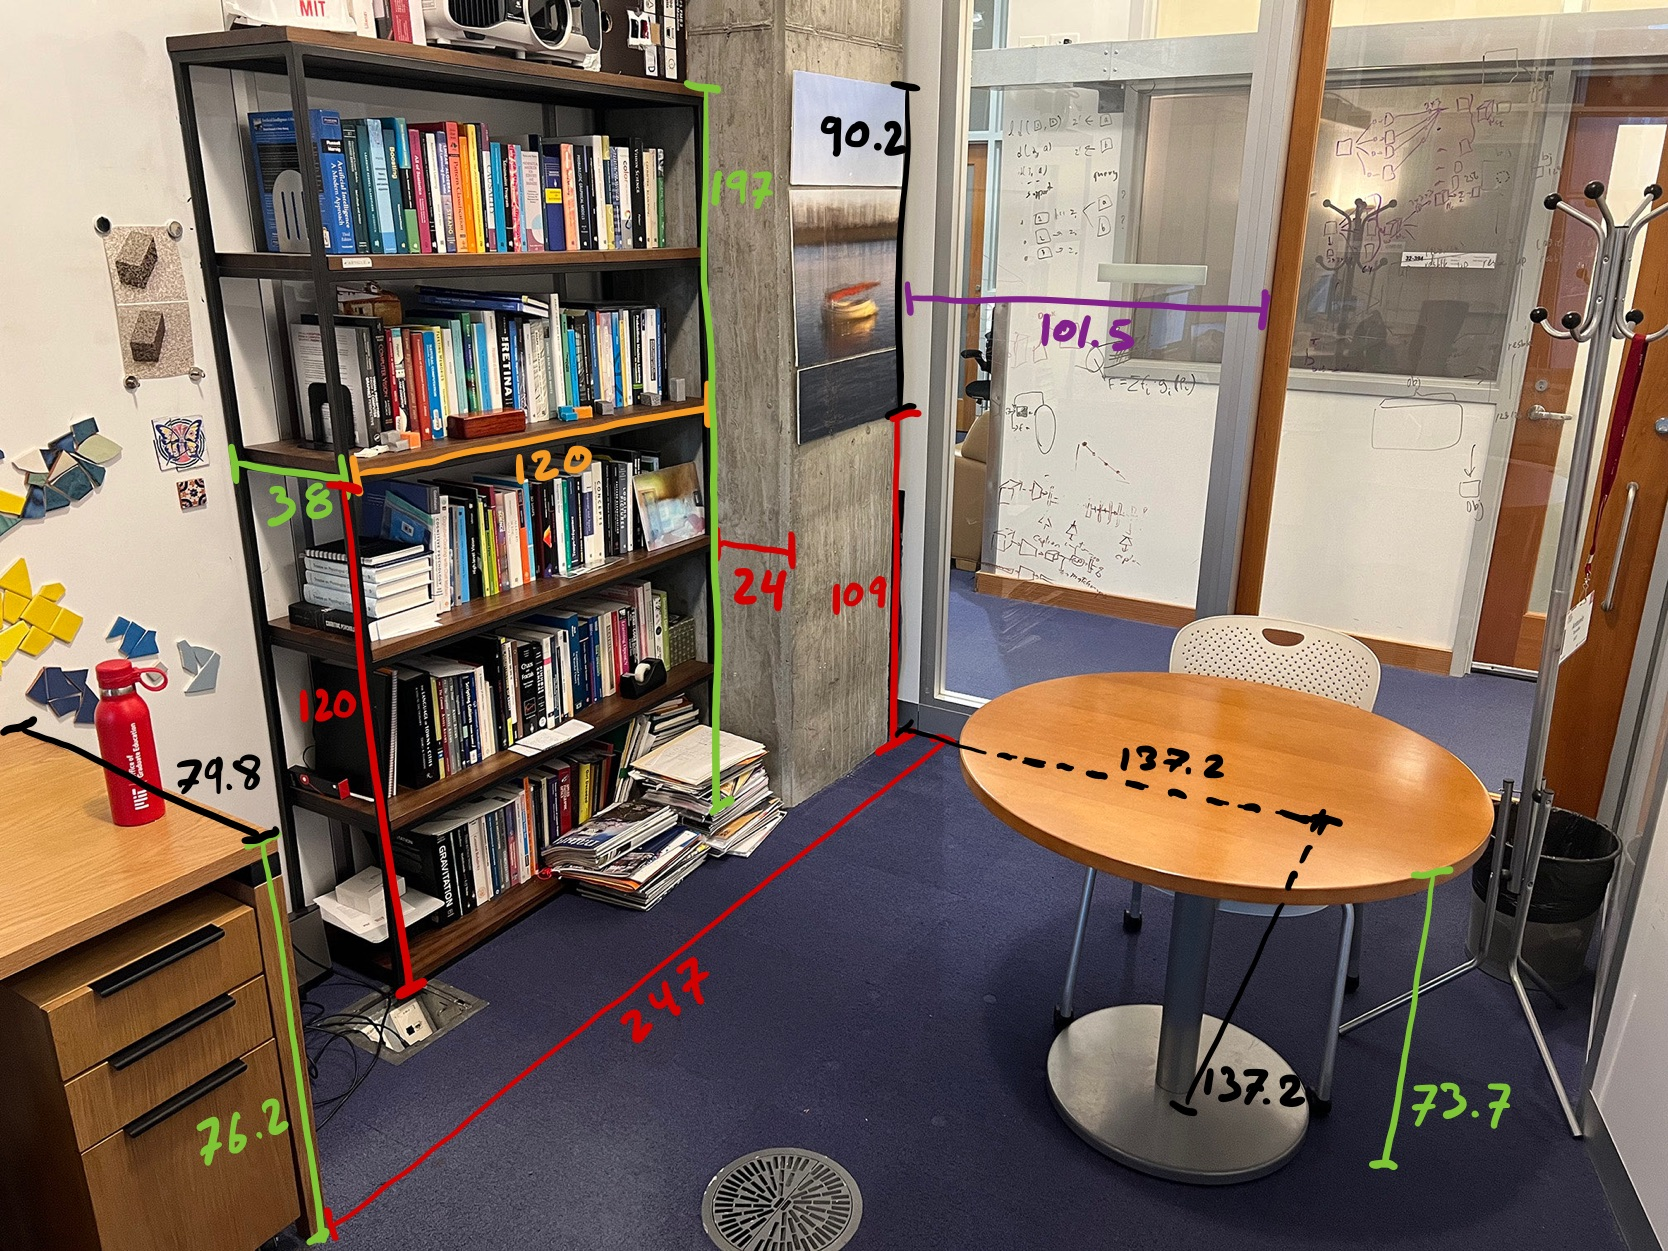
\includegraphics[width=1\linewidth]{figures/imaging_geometry/office_with_measures_2.jpg}
}
\caption{Office picture and real distances between a sparse set of points measured in centimeters.}
\label{fig:office_measurements}
\end{figure}


We took a picture, \fig{\ref{fig:office_measurements}}, with the same iPhone we used in section \ref{sec:simple_unreliable_calibration_method}, holding the camera at eye height (which is around 67 in, or 170 cm above the ground). The camera was looking downward at an angle of around 15 degrees with respect to the vertical. Would we be able to recover these extrinsic camera parameters, together with the intrinsic camera parameters, using the theory described in this chapter?

First we need to decide where we will place the origin of the world coordinates and the axis direction. As shown in the following picture, we place the origin on the ground floor, in the corner between the column and the glass wall in the back.  Now we can get a list of 3D points from the office measurements and their corresponding 2D coordinates. The following figure shows a list of easily identifiable 3D points and their corresponding image coordinates.  The image coordinates are approximated also and are collected manually. We use Adobe Photoshop to read the pixel coordinates. 

\begin{figure}[ht]
\centerline{
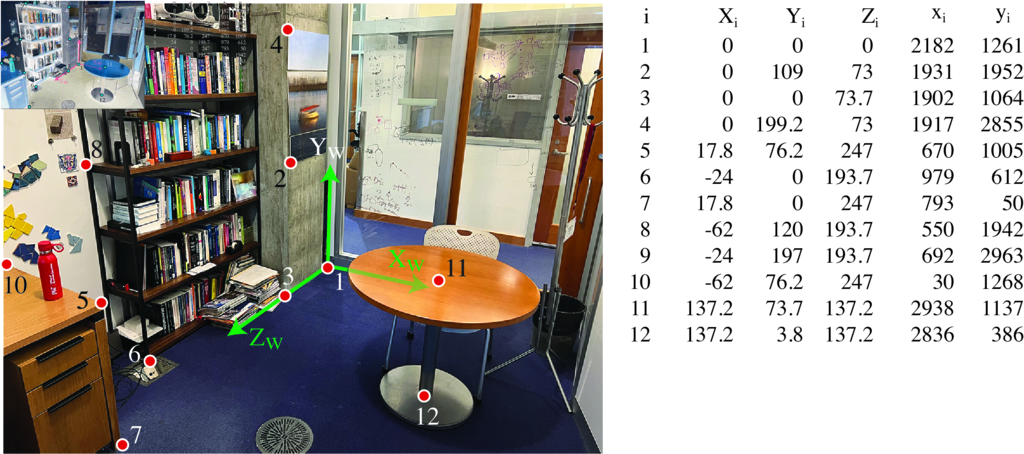
\includegraphics[width=1\linewidth]{figures/imaging_geometry/correspondences_img.eps}
}
\caption{Office picture and a table with the 3D world coordinates of 12 points, extracted using the measurements from \fig{\ref{fig:office_measurements}}, and their corresponding 2D image coordinates measured in pixels.}
\label{fig:office_correspondences_img}
\end{figure}

Photoshop has the image coordinates origin on the top left. Our convention has been to put the origin on the bottom and the $x$-axis point from right to left. Therefore, we need to change the coordinates first (or just deal with it later). It is just simple to replace the image coordinates by $y_i \leftarrow 3{,}024-y_i$ and $x_i \leftarrow 4{,}032-x_i$.

In order to estimate the projection matrix we need a minimum of eight correspondences. Here we have 12, which will help to reduce the noise (and we assure you there is a lot of noise on those manual measurements). Applying the DLT algorithm we recover the following projection matrix:
\begin{equation}
    \mathbf{M} = 
    \begin{bmatrix}
    -8.1    &       -1.8      &     -0.2    &     1{,}845.5\\
      -3    &        5.4      &     -4.8    &     1{,}262.5\\
       0    &          0      &        0    &          1
    \end{bmatrix}
\end{equation}
The matrix has been scaled so that the bottom-right element is a 1. Using this matrix, the mean reprojection error is 12.3 pixels, which is reasonably small for an image of size $4{,}032 \times 3{,}024$ pixels. That is, the reprojection error is $<0.5$ percent of the image height. 

We now need to recover the intrinsic and extrinsic camera parameters.  Using \eqn{\ref{eq:recover_translation}} we recover first the translation vector which gives us $\mathbf{T} = (182.3; 171.8; 347.6)$. From our definition of the world-coordinates frames, the middle element of $\mathbf{T}$ is the camera height with respect to the ground plane. The value of 171.8 cm is very close to our initial guess! Given a scene with known measurements and a picture, one can find out details about the camera and also about the observer. \marginnote{A picture reveals information about the camera and the photographer, even when there is no one on the picture. It is important to keep this in mind when thinking about privacy.}[-0.8in]


Let's now see if we can recover the camera angle and the intrinsics. Using the QR decomposition as described in section \ref{sec:recovering_intrinsic_and_extrinsic}, we get
\begin{equation}
    \mathbf{K} = 
    \begin{bmatrix}
    2{,}960    &      -24.9    &     1{,}979.7\\
       0    &       3{,}019    &     1{,}433.6\\
       0    &          0    &          1
    \end{bmatrix}
\end{equation}
The values are very close to the ones from \eqn{\ref{eq:intrinsic}} which were obtained using a calibration pattern and also from the camera technical specifications. The off-diagonal elements, which would account for a skew pixel shape in the camera, are small relative to the focal length and probably just due to the annotation noise. Also, both scaling factors are very similar, and their difference might just be due to noise. The camera is likely to have square pixels. The last column is the location of the optical image center, as we defined the image coordinates with the origin in the bottom right instead of that in the image center, and is quite close to what one would expect: $[W/2, H/2,1]$.

Now let's look at the camera orientation. The rotation matrix obtained with the QR decomposition is
\begin{equation}
    \mathbf{R} = 
    \begin{bmatrix}
   -0.8576  & -0.0162  &  0.5141 \\
    0.1928  & -0.9368  &  0.2921\\
   -0.4769  & -0.3496  & -0.8064
   \end{bmatrix}
\end{equation}
The viewing direction of the camera can be obtained as $\mathbf{R}^\transpose [0, 0, 1]^\transpose$ (this is the direction of the $Z$-axis in the camera-coordinates system). 
\marginnote{Another potential bug when extracting the camera orientation is to use the rotation matrix instead of its inverse. We defined $\mathbf{R}^\transpose$ as the rotation needed to move the world coordinate axes to be aligned with the camera-coordinate axes.}[-1.3in]
The angle of the camera with respect to the vertically can be computed in multiple ways. Here is one:
\begin{eqnarray}
\arccos \left( [0,1,0] \mathbf{R}^\transpose [0,1,0]^\transpose \right) &=& \arccos (R[2,2]) \nonumber \\
&=& \arccos (-0.9368) \nonumber \\
&=& 20.5 \text{~degrees}
\end{eqnarray}
Here we just computed the camera $Y$-axis and then computed the dot product with a unit vector along the $Y$-axis of the world-coordinates. 
%The $\arccos$ gives us the angle between the two vectors. 
This angle is also quite close to the approximate value that we gave at the beginning of the section. 
   

It is always important to visualize everything to make sure that all is correct. \Fig{\ref{fig:result_toymodel_3dscene_and_estimated_camera}} shows a visualization of the annotated 3D points and the inferred camera location and orientation. The figure shows three different viewpoints. 

\begin{figure}[t]
\centerline{
\includegraphics[width=1\linewidth]{figures/imaging_geometry/result_toymodel_3dscene_and_estimated_camera_b.eps}
}
\caption{Inferred camera location for the office picture. The figure shows three different viewpoints.}
\label{fig:result_toymodel_3dscene_and_estimated_camera}
\end{figure}


\section{Concluding Remarks}

%What are the camera parameters in the output of an image generative model?

In this chapter we have developed a model for describing how points in the 3D world project into the image.
For a more in depth study of the topics described in this chapter, the reader should consult specialized books such as \cite{Trucco1998} and \cite{Hartley2004}.

There are a number subtleties involved in computing the quantities we have presented in this chapter. Although there are packages that will calibrate a camera and compute the projection matrix for you, it is useful to be familiar with how these methods work as they play an important role when building unsupervised learning methods. Unsupervised learning often demands familiarity with the constraints of the vision problem, which become useful when trying to design the loss functions that do not require human annotated data.

But the goal of vision is to interpret the scene, that is, to recover the 3D scene from images. We will discuss in the next chapters how to do this.

 